% wfbook
% wfbook.tex

\documentclass[12pt,UTF8]{ctexbook}

% 设置纸张信息。
\usepackage[a4paper,twoside]{geometry}
\geometry{
	left=25mm,
	right=25mm,
	bottom=25.4mm,
	bindingoffset=10mm
}

% 图片相关设置。
\usepackage{graphicx}
\graphicspath{{Images/}}

% 设置字体,并解决显示难检字问题。
\xeCJKsetup{AutoFallBack=true}
\setCJKmainfont{SimSun}[BoldFont=SimHei, ItalicFont=KaiTi, FallBack=SimSun-ExtB]

% 目录 chapter 级别加点(.)。
\usepackage{titletoc}
\titlecontents{chapter}[0pt]{\vspace{3mm}\bf\addvspace{2pt}\filright}{\contentspush{\thecontentslabel\hspace{0.8em}}}{}{\titlerule*[8pt]{.}\contentspage}

% 设置 part 和 chapter 标题格式。
\ctexset{
	part/name= {第,卷},
	part/number={\chinese{part}},
	chapter/name={第,篇},
	chapter/number={\chinese{chapter}}
}

% 设置署名格式。
\newenvironment{shuming}{\hfill\bfseries\zihao{4}}

% 注脚每页重新编号,避免编号过大。
\usepackage[perpage]{footmisc}

\title{\heiti\zihao{0} wfbook}
\author{WangFei}
\date{\today}

\begin{document}

\maketitle
\tableofcontents

\frontmatter

\chapter{前言}



\mainmatter

\chapter{生殖器官}

\section{女性生殖器官}

女性的生殖器官包括外生殖器官和内生殖器官两部分。外生殖器主要是指阴阜、大阴唇、小阴唇、阴蒂、阴道前庭、尿道口、阴道口、处女膜、前庭大腺和前庭球,而内生殖器则包括阴道、子宫、输卵管和卵巢。

\subsection{外生殖器官}

阴阜在耻骨联合前方,由皮肤及很厚的皮下脂肪层构成。到性成熟期常有阴毛,分布呈倒三角形。

外阴靠近两股内侧的一对长圆形隆起的皱襞为大阴唇。大阴唇外面长有阴毛,皮下是脂肪组织、弹性纤维及静脉丛。生育前大阴唇自然合拢,生育后向阴阜两侧分开。大阴唇内侧有一对小阴唇,是一对黏膜皱襞,表面湿润,有丰富的神经分布,因而感觉敏锐。

阴蒂位于两侧小阴唇之间的顶端,是一个长圆形的小器官,末端为一个圆头,内端与一束薄薄的勃起组织相连接。勃起组织有丰富的静脉丛和神经末梢,是女性最重要的性感区,对其进行爱抚会引起强烈的性反应。

两侧小阴唇之间的凹陷部分是阴道前庭,阴道前庭表面有黏膜遮盖,前半部有尿道开口,后半部有阴道开口。尿道口是一个形状不規则的橢圆小孔,尿液從這裏流出。

阴道口被一塊不完全封閉的黏膜所遮盖,中间是处女膜。处女膜的正反两面都是湿润的黏膜,黏膜之间有结缔组织、微血管和神经末梢,中间的小孔即处女膜孔,经血即由此流出。处女膜孔的大小和膜的厚薄程度因人而异。处女膜破后,黏膜变成许多小圆球状物,成为处女膜痕。

阴道口的两侧有前庭大腺(又称“巴氏腺”),能分泌液体,有滑润功能。前庭大腺有小蚕豆般大小,性兴奋时能分泌黄白色黏液,起滑润阴道口作用。正常检查时摸不到此腺体,如有感染时则会肿大。前庭球又称为“球海绵体”,是一对海绵体组织,位于阴道口两侧,能勃起。

\begin{figure}[htbp]
	\centering
	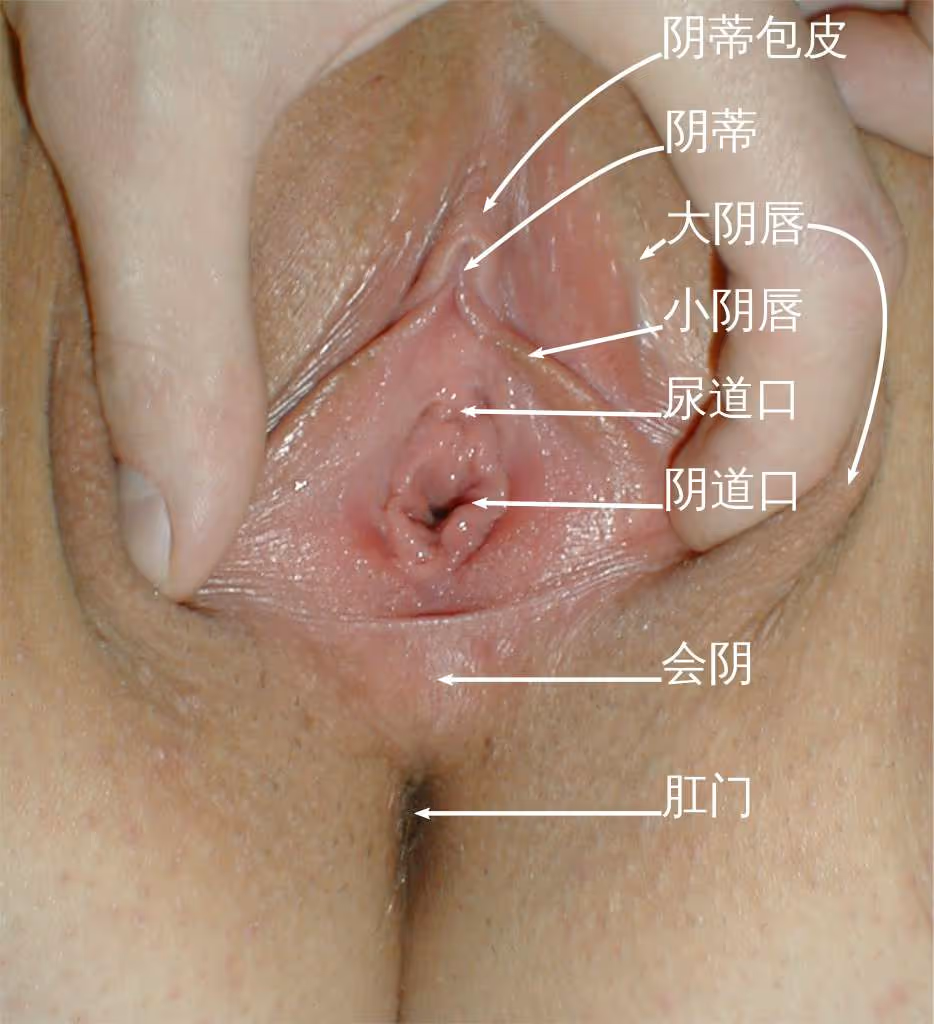
\includegraphics[width=0.7\linewidth]{1}
	\caption{}
	\label{fig:1}
\end{figure}

\begin{figure}[htbp]
	\centering
	
\includegraphics[width=0.7\linewidth]{2}
	\caption{}
	\label{fig:1}
\end{figure}

\subsection{内生殖器官}

卵巢呈卵圆形,位于盆腔内子宫的两侧,左右各一。卵巢发育成熟后,能产生成熟的卵子,并分泌雌性激素,维持女性特征。在一个月经周期中,卵巢内常有几个甚至十几个卵泡同时发育,但一般只有一个发育成卵子。

输卵管位于子宫两侧,是输送卵子进入子宫的弯曲管道。输卵管内端与子宫腔相通,外端游离。输卵管管壁由黏膜、肌层及外膜三层组成。黏膜上皮为单层柱状纤毛上皮。纤毛具有摆动功能。肌层的蠕动及纤毛的摆动,有助于受精卵进入子宫腔内。

子宫位于骨盆腔内,在膀胱与直肠之间,形状似倒置的梨子,前后略扁,分宫底、宫体、宫颈三部分,上通输卵管,下接阴道。
===========================================
子宫是孕育胎兒的器官,又是产生月经的場所。子宫壁共分三层,由外向内为外膜、肌层和内膜。

阴道是一種收縮性很强的肌性管道,上通子宫颈管,下开口于阴道前庭,阴道前壁緊貼膀胱和尿道,后壁与直肠相鄰。阴道为性交器官,又是月经排出和胎兒娩出的通道。

\begin{figure}[htbp]
	\centering
	
\includegraphics[width=0.7\linewidth]{3}
	\caption{}
\end{figure}

\section{男性生殖器官}

男性生殖器官分为外生殖器官和内生殖器官两部分。外生殖器包括阴阜、阴囊和阴莖,而内生殖器由睾丸、附睾、精索、输精管及射精管、精囊腺、前列腺、尿道球腺、尿道等组成。

\begin{figure}[htbp]
	\centering
	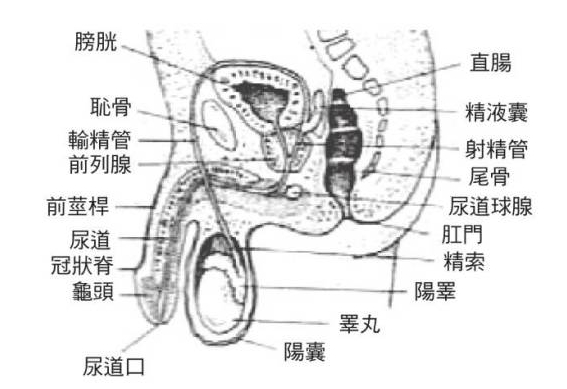
\includegraphics[width=0.7\linewidth]{4}
	\caption{}
\end{figure}

\subsection{外生殖器官}

阴阜为恥骨前方的皮肤和丰富的皮下脂肪组织。青壯年时阴阜顯著隆起,中年以后脂肪组织減少下陷,老年则萎縮变平。

阴囊是由皮肤、肌肉等構成的柔軟而富有弹性的袋状囊,裏面有睾丸、附睾、精索,主要功能有保護睾丸、調節溫度、有利于精子的产生和貯存等。阴囊内有阴囊隔,将阴囊内腔分成左右两部分,各容納一个睾丸和附睾。阴囊皮肤薄而柔軟,并有很多的褶皱。阴囊皮肤有明顯的色素沉著,长有稀疏的阴毛。

阴莖后部为阴莖根,中部为呈圆柱形的阴莖体,其前端膨大部分为阴莖头(俗称「龜头」)。阴莖軸与阴莖头之间是冠状溝,阴莖头与冠状溝含有丰富的神经末梢,对刺激是很敏感的,而冠状溝处神经分布最丰富,敏感性最高。阴莖体由阴莖海绵体和尿道海绵体组成,具有丰富的血管、神经、淋巴管。從外形上看,阴莖有鬆弛和勃起两種状態,具有排尿、性交、射精三大功能。

\subsection{内生殖器官}

睾丸是男性生殖腺,呈卵圆形,左右各一,由精索将其懸吊于阴囊内,长約4~5公分,厚約3~4公分,約重15公克左右。睾丸是产生雄性生殖細胞(即精子)的器官,也是产生雄性激素的主要内分泌腺体。

附睾位于睾丸的后外侧,外形細长,似半月形,左右各一,长約5公分。附睾有儲存和排放精子、促使精子成熟及供給精子營養的作用。

精索位于睾丸上端至腹股溝管腹環之间,左右各一,全长約14公分。精索是睾丸、附睾及输精管血液、淋巴液循環的通路,也是保證睾丸的生精功能及成熟精子输送的主要途徑。输精管是精索内的主要结構之一,其末端与精囊腺的排泄管匯合成射精管,穿過前列腺,开口于尿道,全长約40~46公分,直徑約2~3公釐。

输精管是精子從附睾被输送到前列腺部尿道的唯一通路。射精管是输精管壺腹与精囊管匯合之后的延續。射精管很短,长僅为2公分左右,管壁很薄。

精囊腺为一对扁平长囊状腺体,左右各一,表面凹凸不平呈结節状,其末端細小为精囊腺的排泄管,与输精管的末端匯合成射精管,在尿道前列腺部开口于尿道。精囊长4~5公分,寬約 2公分,容積約4C.C。精囊为屈曲状的腺囊,其分泌液主要为精漿液,占精液的70\%左右,对精子的存活有重要作用。前列腺为一个栗子状的腺体,平均重量約20公克,是男性最大的附属腺体,能分泌前列腺液,组成精漿液。前列腺還被認为是一个性敏感部位,对其进行適當刺激时,可以引起性兴奋。尿道球腺左右各一,位于尿道生殖隔上下筋膜之间的会阴深囊内,开口于球部尿道近端,可分泌少量液体,为精漿的成分之一。

男性尿道长12~20公分,既有排尿功能,又有排精的功能。

其中有尿道球腺,可分泌液体,參与精液的组成,性交时有润滑阴莖头的作用。

\chapter{性慾}

簡单地說,性慾就是对性生活的一種慾望,它既受体内激素水準的調節,也受社会、家庭等周圍環境因素的影響。同时存在比較大的个体差异,即使是同一个人,性慾的高低也隨年齡、心理状態、患病状況、生活品質、工作環境、婚姻状態等不同而表現不同。

一般情况下,性慾源于性心理的驅动,比如对异性的爱慕可以誘发性慾。男女之间建立美滿家庭以及夫妻间的親暱,都会产生性交的慾望。性慾产生的另外一个原因与内分泌有關。青春期過后,驟然提高的人体性激素分泌水準会驅动性慾。男性精囊、前列腺等性腺内分泌物的增加与淤積,女子外阴前庭大腺等分泌物的過多貯存,都可誘发性刺激和促进性慾。此外,既往性生活的愉快感受,或者男女之间身体接觸产生的性刺激等,也可以誘发性慾。所以,性慾是多方面因素綜合作用的结果,不但思维、意識、情感、環境等因素与性慾相關,而且語言、文字、圖畫、音樂等,也会給性慾帶來舉足輕重的影響。

\section{男人的性慾和女人的性慾一樣嗎}

從表面上看,男人的性慾似乎比女人强,因为在性生活中居于主动地位的女性比較少,這裏面既有生理上的因素,但主要還是心理因素的影響。许多女人習慣于壓抑自己的性需求,所以,在多數情況下,男人的性慾表現得比女性主动,但這不證明男人的性慾就比女人的性慾强。

处于青春期的男性比女人更富于性幻想,并容易將感情需要和性需要混为一談。成年以后,工作的壓力和家庭的負擔,会使青春期旺盛的性渴望減弱,但仍有少數人性慾一直比較强烈,在這一點上,女人和男人是一樣的。男性的性慾在某些年齡階段表現得要比女人强,但在另一些年齡階段卻可能完全相反。在性生活不和諧的夫妻中,产生性慾低下的一方往往是丈夫,其中年齡是个重要因素,男人的性慾高潮期通常在30歲以前,而女人则是在40歲左右,才对性活动表現出濃厚的兴趣。

\section{为什麼有的人性慾强,有的人性慾弱}

性慾是有很大的个体差异的。性慾的强弱程度与下列因素有關:

①遺傳因素:性慾的强弱程度受遺傳因素的影響,一个家族的成員,往往表現出類似的性慾傾向。

②激素水準:人体中有多種激素,男女皆然。在多種激素中,雄性激素对性慾的影響最大。雄性激素水準高,性慾就强,雄性激素水準低,性慾就弱,無論男女都一樣。

③感觉刺激:在多種刺激下,人体就会产生各種各樣的感觉,如視觉、味觉、聽觉、嗅觉、觸觉等,這些感觉可以激起性慾,在這一點上男性和女性沒有明顯差异。

④性体驗和性经驗:如果以往性体驗順利并且性经驗丰富,性喚起就比較容易;反之,性慾的产生就比較困難。

⑤環境因素:人体会对外界環境的刺激作出多種反应,所以生活環境中的光照、溫度、濕度、季節、飲食等因素,都会影響性慾的产生。

⑥文化因素:性慾的产生是一種个人行为,但性慾也与文化因素有關,在某種程度上它必須接受倫理、法律、道德,甚至醫學的約束。

⑦情緒变化:心理状態影響著性慾的产生,比如當人們被憂慮、恐懼、憤怒、抑鬱、疼痛、痛苦所困擾的时候,一般是很難产生性慾的。

⑧年齡因素:人的性慾会隨著年齡的变化而变化。就一般規律而言,男性的性慾高峰在30歲之前,而女性则是在40歲以后性慾最为高漲。隨著年齡的增加、内分泌的改变,体内雄性激素的減少,人体感觉会变得遲鈍,導致性器官血液循環不良,再加上來自事業、生活及社会交往等方面的壓力,這些因素都会使人的性慾減
退。

⑨健康因素:健康的生理状態是维持性慾的基礎。人体的各種疾病,如内分泌、生殖器官、代謝系統、肿瘤及其他消耗性疾病,都会影響性慾的产生。

總之,性慾是人的生理本能之一,它受多種因素的影響。

\section{不要將性慾望和性功能混为一談}

現實生活中,不少人对性都存在認識上的誤区,將性慾望和性功能混为一談即是其中之一。實際上,這两者還是有区別的。

所謂性慾望是对性的一種要求、一種渴望的心情,而性功能则是將慾望化做具体行为的能力,完美和諧的性生活,需要性慾望和性功能的協調和統一。如果能將性慾望和性功能協調于一身,就能充分享受性所帶給自己的愉悅;但是要想實現這个願望,需要不斷地摸索和探尋,如果沒有完成這種轉化,就会導致性的各種不和諧和性功能障礙。

實際上,性慾望和性功能分离的情況是很常見的,常見原因有生理性的,也有精神心理性的,還有疾病等因素。比如,进入青春期的青少年,开始出現朦朧的性意識,也具有了阴莖勃起的能力,但他們对性的慾望還沒有建立起一个明確的概念;一个習慣自慰的青年,有可能擔心自己患了陽痿,懷疑自己的性能力;老年男性,儘管歲月的磨煉使他們更加珍爱生活、珍爱爱情,对于性的要求(慾望)也很高,但是性功能卻在慢慢地減退,直至消失;患有某些疾病的男子,儘管主觀上很想「要」,但實際能力卻不行;某些傳染病患者,儘管性功能很好,但为了疾病的康復,必須抑制自己的性慾望。

\section{性生活不僅僅意味著性交}

性生活是夫妻间表達感情、傳遞爱意的重要手段。在正常的夫妻性生活中,即使男性最終出現了高潮和射精,但這也并不是性生活的全部内容,更不是它的首要目的,性生活還包括夫妻雙方的精神交流、性生活中的默契配合和性交后的恩爱,性生活的品質,在很大程度上,取決于全部過程的圆滿程度。

有些人常把性交過程看做是第一位的,于是導致了性生活的過于急切、粗暴和簡单的程式化。丈夫容易忽視妻子的情感需求,把性生活簡化成一系列的动作,甚至有人为了顯示自己“性能力强”,而粗暴地强迫妻子与自己過性生活,極大地傷害了妻子的人格与情感。這種「性」多、爱少的方式,只会給对方帶來痛苦和厭惡,而不是身心愉悅。其實多數女性最看重的并不是性交的過程,而是相互溫存的感觉与感情交流。

有關調查顯示,夫妻中大約有四分之一的人几乎從不相互親吻;差不多有一半的男性很少抚摸妻子,但他們均認为自己的婚姻生活是和諧美滿的,或者是比較滿意的。由此可見,多數男人往往是過分地偏爱最終的性交過程,這種現象在鄉下更为普遍,有些人只是把性看作是一種生活内容,是必須履行的義務,而不是为了傳遞爱。

現實生活中,家庭、職場有很多問題都要面对,身心疲憊的情況会时有发生。如果夫妻中的一方想要過性生活,而另一方则状態不好只是勉强为之,那麼性生活结束之后,不僅主动的一方会觉得毫無兴致,而被动的一方也会更加難過甚至痛苦,長期下去会形成惡性循環。事實上,越是突发地匆匆行事,就越是極其狹隘地理解性生活的内容,也就越缺乏交流和深切感受,身心疲勞也就越是加重,结果把性生活变成消極、冷漠和缺乏激情的「機械化運动」,夫妻雙方難以体会性生活帶來的愉悅感,甚至出現性功能障礙和性冷淡,并由此喪失了爱心、情趣及性的和諧之美。過去這種情況在中年男人身上比較多見,但近些年一些年輕人,甚至新婚不久的男性也抱怨「沒意思」,其實是同樣的原因所導致。因此,無論男人還是女人都应該切記:为了爱而性交,而不是为了性交而性交。把握好這个基本點,一切的問題也就順理成章地容易解決了。

\section{性交时应適时插入}

性交是夫妻生活的重要内容,關係到夫妻感情的和諧与否,所以夫妻雙方不应草率從事或敷衍应付,在性交前要做好充分的準備工作。在性刺激下,男女雙方的性器官都会逐步处于充血状態,男性阴莖膨大了,女性阴道也有变化,但這些变化所需的时间,男女有很大的差异。當男性的性慾達到一定的程度,阴莖勃起变硬时,多數男人著急要进入下一步工作,但女方性慾的激发,往往需要一定的时间,短的需要几分鐘,長的可在半小时以上。當然,有性交经驗以后,夫妻之间的差异会縮短,并基本保持一致。

性交时男女雙方的体内,都会分泌出具有润滑作用的液体,有助于激发性兴奋。此时男性阴莖上端的阴莖头被润滑的液体所滋润,女性阴道外及阴道内壁也都分泌著這種物質,男性阴莖靠著這些润滑的液体,插入女性阴道会变得容易,但是如果男性性急,在這種润滑的液体分泌之前,便要插入女性的阴道,再加上动作粗暴,不但容易使女性受傷,也会使女性产生恐懼性交的心理,還会給自己的性器官帶來明顯不適(疼痛甚至損傷),給以后的性生活造成障礙。所以在性交前做充分的準備工作是非常重要的。

\section{怎樣理解性快感}

性快感是性生活中的一種心理感受,雖然目前還沒有具体的量化指標,但界定它的程度,可以從以下几个方面去体驗它的存在。

首先是宣洩后的輕鬆感。男性在性刺激下产生性兴奋,阴莖勃起,产生交媾的慾望,達到射精。射精之后恢復平静,心境弛緩,獲得宣洩后的滿足,這是性快感的内容之一。

其次是夫妻情感的交匯融合。夫妻恩爱,相互溫存相偎,进行爱抚,引发性衝动而进入性高潮。性高潮之后,雙方进一步溫存、体貼,会产生一種发自内心的愉快。

性快感的另一内容是在疲勞中体会快樂。從性兴奋的产生到最后射精结束,雙方都有高强度付出后的疲勞感,這種疲勞感其實也是一種無聲的交流,其产生的快樂是其他事情難以取代的。

總而言之,性快感不僅僅是性器官的感觉,必須從情感、心理和行为中去感受它的存在。单純的性宣洩是粗野的行为,是不可能产生完美快樂的感觉的。

\section{性生活的几个階段}

性生活大体有四部分的内容,即性交的預備、性器的交合、性行为的運动、性交的结束。這个過程又可以分为兴奋期、平臺期、高潮期和消退期。

①兴奋期:在肉体或精神上的性刺激下,性慾被喚起,身体开始处于緊張階段。

②平臺期:即性高潮前期,在這个階段的基礎上,身体的性緊張逐漸到達顶峰。

③高潮期:持續时间很短,大約只有几秒鐘的时间,高度緊張的肌肉经過痙攣,处于放鬆的状態,使人獲得快感。

④消退期:身体由緊張逐步鬆弛和消散的過程。

性生活的不同階段,男女雙方的身体都会出現相应的生理变化,但是這種变化是存在很大的个体差异的。

\section{射精和精液的主要成分}

男性在性高潮或遺精时,精液通過输精管、精囊、射精管、精阜开口及尿道被排出体外,這便是射精。

\begin{figure}[htbp]
	\centering
	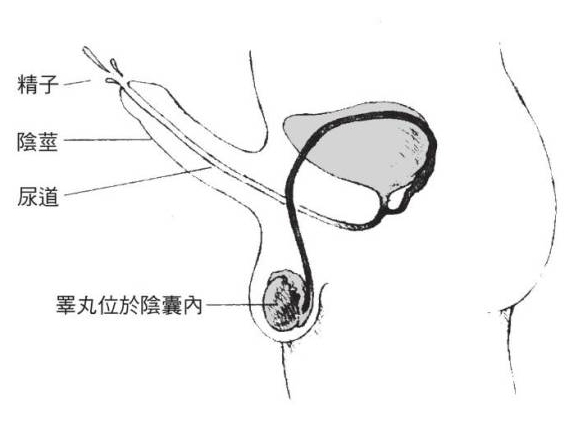
\includegraphics[width=0.7\linewidth]{5}
	\caption{}
\end{figure}

一般情况下,一位男性每次排出的精液为2~6C.C,每C.C含成活的精子为6千萬~1.5億个左右。精液是由精子和精漿组成,精漿又包括前列腺液、精囊液和尿道球腺液等成分,其中前列腺液約占三分之一,精囊液約占三分之二。精漿負責输送精子,并为精子提供能量和營養物質。精漿中主要成分是水,此外還有糖類、電解質、酶類、维生素等物質,這些營養物質是保證精子生存与活动的物質基礎。各種液体射出的先后順序为:首先射出的是約0.1~0.2 C.C的尿道球腺液,接著射出的是總量約0.5C.C的前列腺液和精子,最后射出的是約2.0~2.5C.C的精囊液。

\section{男性怎樣判斷自己的性功能}

性功能是人類的基本本能之一,在生活中的地位是不容忽視的。健康、完善的性功能,不僅是身体健康的標誌,而且還影響著人的精神状態、生活品質、生育后代的能力,以及人格魅力等方面,同时也是性文化中不可缺少的一部分。

怎樣判斷自己的性功能、如何对待自己的性功能,如果缺乏必要的知識積累,難免会走入誤区。比如,有的人一旦发現自己的性能力出現一些变化就憂心忡忡,陷入焦慮和困惑,懷疑自己是不是性功能減退了,終日疑神疑鬼,亂吃補藥,或者偷偷地去找江湖庸醫,结果問題不但沒有解決,還引发了別的麻煩。事實上,相當一部分懷疑自己性功能有問題而前去就醫的「患者」,在经過相關的醫學检查后,并沒有发現有什麼疾病,所謂的性功能減退,實際是過度緊張造成的。

還有一些人与上述這些人不同,他們一旦发現自己的性功能有問題,「死要面子活受罪」,遲遲不肯看醫生,長期生活在巨大的精神壓力下,當情況发展到非常嚴重的地步、不得不就醫时,往往病情已经很嚴重,治療起來自然相當困難。

怎樣正確評價自己的性功能呢?以下几點供參考:

(1)關注性器官的勃起状態

年輕且身体健康、精力旺盛的人無論何时,一旦有性方面的刺激,都会对性产生兴趣,阴莖能迅速勃起;年紀稍長一些的中年人,可能会在勃起之前需要一段时间,這些都是正常的。但如果你发現自己的性器官有时候勃起,有时候不能勃起,或者雖能勃起,但堅持不了多長时间,未到射精时就疲軟下來,這種情況常常提示你的性功能可能有所降低,但問題不大,可以通過適當的食補、正確的藥補,及科學的鍛鍊进行糾正。比較嚴重的情況,是在較長的一段时间裏,阴莖始終沒有勃起過,這就需要看醫生了,应該到醫生那裹接受检查后,再採取相应的措施。

(2)判斷自己性慾产生的方式

性慾比較旺盛的人,一般都会在性生活中处于主动地位。在有些两性關係中,如果男女雙方的性慾强度差不多,常常是男女互为主动,當然也不排除女方主动的情況。如果女方主动,男方能夠積極回应,就大可不必为自己的性功能擔心。如果你在性生活中表現得很消極,必須依賴对方的主动,或者即使对方主动誘導,也很難激起你对性的兴趣來,說明你的性能力出現了問題。

性能力出現問題,不要消極迥避,積極的应对措施是尋求專業醫生的幫助。除了男科醫生外,諮詢心理醫生也是十分必要的。如果沒有器質性疾病,措施得當,問題并不難解決。只是一定要科學就醫,而不是消極迴避或「有病亂投醫」。

3)对性的關心程度是性功能的一種表現

性功能包括性生理和性心理两方面的内容。一般情况下,性心理和性生理正常的男性,無論年齡多大,一旦看見性感、年輕、漂亮的女子,都会情有所动,看見妻子裸露的肌肤,「肤色如凝脂」,就会有想抚摸的衝动,這是正常的性反应,不能一概歸结为「下流」。如果遇到和自己關係很親近、很鍾情的女性,只能产生一般的交談所帶來的快樂,而不产生任何性的想像,說明你的性感受开始变得遲鈍了,需要想辦法去提高自己的性兴奋程度,像治療軀体的其他疾病那樣,尋找病因,进行对症治療。

\section{適时变换性交姿勢}

经過磨合之后,夫妻性生活时的姿勢往往就固定下來了,久而久之,可能一如當初时那樣美滿,但也可能由于一成不变的固定模式,導致性生活品質下降。正確的做法是偶有变化,雖然并不一定嘗試每種姿勢。

性交姿勢又叫性交体位,对性反应的性質和强度,都有很大的影響,如果性交体位不適宜,就会造成性兴奋程度的下降。沒有哪一種体位適合于所有的配偶,因此要对其进行探討。夫婦雙方的性器官未必十分吻合、貼切,有大、小方面的不適应,要根據這種不適应用不同的体位來補救,并找出最容易達到性高潮的体位。由于性交体位的改变,有助于提高性生活的品質,所以夫妻雙方要密切配合,找出更理想、更適合于自己身体條件,和更有利于性感滿足的新姿勢來,比如可以在一次性交過程中,由一種体位变換到另一種体位,甚至变換好几種体位。常用的性交体位有如下几種:

(1)男上女下(女仰臥、男俯)

這是最傳統、最常用的性交体位。隨著歷史和性文化的发展,人們的人文理念、文化修養、社会習俗,都早已发生了深刻的变化,「男上女下」已不是唯一「正統」的性交体位,人們勇敢地进行著新的嘗試,但「男上女下」的体位,仍然被许多人所崇尚和實踐著。

「男上女下」的体位,自有其被推崇的理由,但仍有些女性感到男上式限制了她們的活动,另外一些女性则認为這一体位比較舒服,女子正面的乳房、阴阜承受壓力,能产生出觸觉快感。

(2)女上男下

這種体位能更好地发揮女方在性生活中的主觀能动性,因为它在很大程度上,可以由女方自己來控制性活动的进程,比較適合性感超常的女性。此外,喜歡追求刺激性的女性,採用「女上男下」式更易于獲得性滿足。「女上男下」式能使女方子宫下降,阴道口变寬,所以,即使是阴莖短小的男性,也能給女性比較强烈的刺激,使雙方都得到愉悅。

但「女上男下」的体位,不利于对阴蒂的直接刺激,如果女性的会阴口太靠后,或者女性比較肥胖、身体過于龐大笨重,或者女性缺乏经驗时,這種体位也会有一些不足。

(3)侧位

將面对面式稍加以修改即为侧位,即女方侧臥,男方面向女方在其两腿之间躺下。這種体位既簡单又易于掌握,也十分舒適,因为雙方的身体重量基本都壓在床上,彼此負重很少,便于保存体力,不会感到勞累。由于這種体位使雙方的骨盆向各个方向的活动,都不大容易受到限制,特別是女性可以自由活动,便于掌握節奏,同时還有利于男方对射精的控制,以及用手來刺激女方乳房、阴阜及阴蒂等部位,所以適宜在妊娠期使用,它可以避免对胎兒的壓迫,是比較可靠的方法。

(4)后进入式

是男性面向女性背部的一種体位。這種体位可以十分方便地用手对阴蒂进行直接刺激,這樣就造成了对阴道区域的更緊密的觸动,和施加更大的壓力,尤其適合男女雙方都很胖的情況。這種体位也適用于妊娠期。缺點是插入不完全,常会使雙方都感到生理上的緊張,不像面对面时,雙方能夠親密無间地进行擁抱和彼此爱抚。另外,由于阴道入口是由下而上,与阴莖方向相反,可能会給插入帶來一定的難度,但一旦插入,其对阴道的刺激也是很强烈的。

\section{和諧的性生活在于高潮的「同步」}

在性生活中夫妻「同步」達到性高潮,是所有夫妻都嚮往和渴望的。然而現實生活中有不少结婚多年的夫妻,都沒能達到性和諧的程度,如果這个問題处理不好,可能会影響夫妻感情。

和諧的性生活,不僅可以滿足雙方的性慾望,還有利于夫妻的身体健康。所以·夫妻应該爭取享受這種性生活最高境界的「同步」。但是,影響性爱達到理想境界的因素十分繁多,可能有相當部分的夫妻,終生刻意探索也沒能如願,可能是他們太過緊張、執著,限制了对性生活的細緻体驗和充分发揮。

要想達到性生活的和諧,首先要嘹解男女在生理上的差別。男人性慾强·衝动出現快,消退也快,性慾主要集中在生殖器官上,发生性衝动进入兴奋期即急于性交;女人性衝动出現較慢,性慾兴
趣廣泛,需要丈夫的爱抚親吻,性憋产生、增强是達到性和諧的前提。

性爱是两个人之间的事,应該如何进行性和諧的探索,是很个性化的問題。彼此之间的感觉舒服是最重要的,至于要如何做则沒有一定的規则可循,只要两人都能好好享受即可。

下面的一些建議,或许可以起到鬆弛緊張神经的作用,使男女雙方獲得意想不到的滿足感。

①性生活前要做好充分的準備,男人可以採取各種方法來激起妻子的性慾,只有在妻子真正进入了性兴奋状態,性生活才容易獲得滿意。

②丈夫切忌性急和粗魯,絕不可只顧滿足自己而不顧妻子的意願。男人要學会控制自己達到高潮射精的时间,可以通過放慢節奏來實現,因为性不和諧,往往來自于女性的高潮出現較晚,女方也不要勉强应付。

③儘量放鬆,慢慢地体会性過程所帶來的感受和体驗,而不要把自己的注意力,完全集中在追求性和諧上。

④在性生活過程中,把握自己的每一个舉动,讓你逐漸地接近理想境界。

⑤男方把自己的感受告訴妻子,得到妻子的理解、支持和有力的幫助,雙方互相尊重、互相体貼、配合默契才可以達到性和諧。

⑥男性射精后不要立即结束性器官的接觸,還要撐持、与妻子交談,待妻子達到高潮并性慾完全消失,共同结束性生活。夫妻雙方都得到了滿足,這樣才能使性生活和諧起來。

\section{實現夫妻性和諧的必備條件有哪些}

美好和諧的性生活,需要靠夫婦雙方共同努力來實現。为了達到這樣的目的,男女雙方必須要熟悉自己的和对方的性特點,并具備下面這些條件:

①雙方的心理状態良好。夫妻要恩爱,在感情上水乳交融,能創造和諧的性生活氣氛;宜選擇環境安静、心情歡快的时候进行性生活。雙方在性生活中应主动、默契地配合,密切協作,共同充當「二重奏」的主角。恩爱的夫妻關係是性生活和諧的關鍵。

②雙方的生理状態良好。性生活前应进行局部的清潔衛生,清除局部不適因素,增加局部润滑感,這是性生活和諧的必要條件。

③雙方体魄强健,精力充沛。雙方生殖器发育正常,是保證性器官接觸、獲得正常性刺激的生理基礎。選擇身体健康的时候进行性生活,能两情歡愉,如魚得水。

④掌握科學的性知識。正確掌握性生活的四个性反应周期,根據男方性衝动較快、女方性衝动較慢的特點,男方多刺激女方动情并要耐心等待,等到女方有性兴奋后再开始交接,可使雙方的「性慾高潮曲線」趨于重疊,達到男女雙方性生理上趨于同步。

夫妻间性不和諧的主要原因是性知識的缺乏,例如缺乏必要的性知識、不会性交、不会摩擦抽动阴莖、不知道对方的性反应特點、不關心对方的性反应等,因此雙方無法完美配合,性生活也就難以達到和諧的境界。

性和諧以及对性和諧的要求,在不同的夫妻之间是有著明顯差异的。要想獲得和諧的性生活,只有夫婦雙方的積極性同时調动起來,共同實踐、探討、交流,才能共同達到性爱的完美境界。

\section{爱侶间永保性爱和諧美滿的秘訣是什麼}

美滿和諧的性生活,有賴于爱侶雙方情感的交融,将性爱与情爱融为一体,包括以下几个方面的内容:

①婚前注意彼此检點。许多婚后的性与情感的不和諧,都与婚前的性行为或性经驗有關,是導致夫妻生活不和諧的禍根。

②婚后避免缺乏新意和激情的性交。切忌「千篇一律」的性生活,不要为了性而做爱,而应該为了爱而做爱。共同創造新生活,不斷地变換做爱的環境、地點、姿勢和体位,這樣做才可能不斷地密切夫妻间的關係,使婚姻能经受住風雨的考驗。

③要体諒对方。在对方不能滿足你的生理要求时,不要太過計較,過多的責備是要傷感情的,而過分的强求生理滿足,可能使对方厭倦性交,甚至出現各種各樣的性功能障礙或性冷淡。

④能夠達到肉体与精神的和諧美滿。這當然是爱的重要表達方式,但絕对不是唯一的方式,爱的表達形式体現在生活中的點點滴滴。所以,平时要经常表達自己对配偶的爱意,充分体現自己的魅力,为爱創造溫馨的氣氛,而不是只在做爱的时候才进行情感的溝通。

\section{真爱不需要太多的技巧和藝術}

情爱与性爱是密不可分的,情爱可以啟动性爱,而性爱又可以反過來强化情爱,無論单純地强調哪一種爱,都有失偏頗。在現實生活中,有些人往往過分地强調了性爱,尤其是性交的技巧和藝術性,强調了性交动作、姿勢和花樣上的翻新,强調了性爱的創造性,强調了性爱的品味、品質、檔次和環境,這樣做真的有必要嗎?

由于傳統文化的影響,多數人都持有這樣一種觀念,即性生活是否美滿取決于男方,尤其是男方在性生活中的技巧如何,因此把注意力全部集中在有性感受器官的身体部位上。其實,性反应涉及眾多的生理和心理反应,儘管其中的一種或几種可能起著重要的作用,例如性交過程中全身肌肉的緊張度,但其他的反应也是不可或缺的,例如强烈的情爱表達和流露。

我們承認,科學地掌握性技巧是个前提。

①要雙方絕对自願并真正需要,否则將是侵犯对方的人格尊嚴,而且会造成雙方的心理傷害,也不会产生好的效果。

②夫妻感情良好。

③雙方性知識和性態度的水準非常接近,彼此容易溝通和接受对方的安排。

④所用的性技巧必須是具有科學性的,并要準確掌握其適用範圍,這樣性生活才会产生有益的效果。但性技巧本身既不能製造爱情,也難以充分地溝通夫妻间的感情。如果過分强調性技巧,会对感情产生不良作用,使性爱的行为变成一種機械的动作,極易導致雙方或一方产生疏遠、孤獨、人格受侮辱等不良情緒,削弱了性爱与情爱之间的必然聯繫。

真爱不需要太多的技巧,讓性慾順其自然地发洩就是最好的,如果人工「製造」性爱的味道濃了,性爱的負擔也就产生或增加了,緊張焦慮情緒也就出現了;而隨心所欲、順其自然的自然发揮也就少了。

正处在精力充沛、激情亢奋階段的青壯年男人,完全可以要風得風、要雨得雨,沒有必要尋找所謂的性爱的感觉和性爱的技巧,隨意发揮都是真情的流露和刻骨銘心的記憶;处在激情不再階段的中老年男人,也应該是坦坦然然,平平淡淡才是真,跟著感觉走的感觉最好,而不需要刻意强求。實際上,最高級、最通用的「性技巧」不是动作上的而是心靈上的,是盡可能多地把爱慕、依戀、親密和關心之類的真情傾注和濃縮于性生活之中。

所以,迷信性技巧而又忽視情感交流的人,其實是在自討苦吃。做爱不要太苛求自己,不要太講究技巧和藝術,只要自我感觉不錯、跟著感觉走就行了。

\section{不宜過性生活的几種情形}

性生活是已婚男女天经地義的快樂享受,性生活的快樂程度,取決于夫妻雙方是否全身心投入和彼此是否傾心配合。此外,不適當的環境、情緒、身体健康状況等因素,都可能限制人們隨心所欲地进行性生活。一旦出現以下几種情形,应該避免性生活:

①生病。儘管疾病并不是性生活的对禁忌,但是在患有某些嚴重疾病,或者疾病的急性期内,一般是要禁止性生活的。因为性生活会对患者自身的健康和疾病的恢復,構成一定的威脅。慢性疾病或者疾病的恢復期内是否能夠過性生活,需要獲得醫生的指導意見。患有性病的夫妻,一定要在性病治癒之后,并渡過了傳染期,才可以過性生活,否则勉强過性生活,受害者不僅是自己,還会通過性器官的接觸,而將疾病傳染給对方。

②過度疲勞。性生活是要消耗很大体力的,且身体或精神疲憊时過性生活,往往不容易達到高潮,收不到雙方滿意的效果。勞累后立即過性生活,還会損害健康,并容易誘发早洩、遺精、陽痿等性功能障礙。

③心情不佳或心緒不寧。有些夫妻在一方情緒不佳或心緒不寧时勉强過性生活,不但得不到性生活的美滿和諧,還会使情緒不好的一方对此产生反感,引起夫妻感情不和;如反覆发生類似情況,還会導致女子的性冷淡或男子的陽痿或其他疾病,例如夫妻因为生活瑣事吵嘴后、夫妻問由于擔心懷孕而顧慮重重等。

④酒后。一些人習慣酒后行房事,有人甚至認为酒后過性生活会「提高品質」,能延長性交时间,尤其是一些早洩患者。其實,酒后,尤其是大量飲用烈性酒后,性生活会造成许多危害,例如射精疼痛、血精等,還可以導致性功能多種障礙,最終会妨礙性生活和諧,而且如酒后受孕,還会給胎兒帶來負面影響。

⑤不講衛生。性器官的衛生状況,直接關係到夫妻雙方的身体健康。生殖器官的不清潔,可以將細菌等病原体帶入对方体内,構成了对健康的威脅;反之,清新、整潔的衛生状況,不但有益于夫妻雙方的健康,還可以增强性感受,有助于性生活的和諧和美滿。

⑥準備不充分。性生活前的準備,是夫妻间心理和生理进入「状態」的必要階段,不可或缺。如果倉促进行性生活,并草率收兵,不僅難以讓妻子達到性高潮,甚至会給她帶來痛苦,久而久之会使她对性生活喪失兴趣,是产生性冷淡的主要原因。

⑦飽食或饑餓时。飽食可以使胃肠道充盈,大腦及全身各个器官(包括性器官)相对地血液供应不足,影響阴莖的勃起程度,故不宜在剛剛吃完飯后就過性生活;饑餓时人的体力下降,精力不充沛,此时過性生活也往往達不到滿意的效果。

⑧精神過度緊張、抑鬱、焦慮。精神極度緊張、抑鬱和焦慮,易引起男性的早洩和陽痿,或女方的性交疼痛(阴道痙攣)。所以,夫妻性生活时,要儘量保持輕鬆、愉快的心情,這樣才能保證性生活的品質。

\section{什麼是性激素}

男性的睾丸和女性的卵巢都是性腺,其分泌出的与人体性器官发育和性功能等有密切關係的類固醇樣的物質,即性激素。男性性激素主要是雄性激素,即睾酮;女性性激素主要是雌激素和孕激素。它們直接进入血液发揮不同的生理作用。

性激素的主要作用有:

①促进性器官发育并维持其成熟状態。雄激素可促进男性性器官发育、成熟,并维持其成熟状態;雌激素可刺激和促进女性子宫、输卵管、阴道、外阴等器官的发育、成熟,并维持其成熟状態。另外,卵巢产生的孕激素与雌激素,能協同完成調節女性的月经周期和生育過程。

②促进第二性征的出現。睾酮具有刺激男性鬍鬚生長的作用,因此,男性会長鬍鬚。睾酮能促进蛋白質合成,使人肌肉发達。雌激素能促进女性皮下脂肪沉積,使其皮下脂肪丰富。雌激素可促进乳房的腺管增生,孕激素可促使乳房的腺泡发育,因此,女性的乳房会发育得較大。睾酮還有促使男性喉结增大、聲帶增厚的作用,所以男性发音会顯得低沉。正因为男女性腺不同,睾丸和卵巢产生的内分泌激素不同,因而各自会出現不同的性特征。

③维持性功能。性激素能引起性中樞兴奋。男性缺少睾酮或女性缺少雌激素,均可引起性慾減退或性功能障礙等。男性嚴重缺乏睾酮,可使精液量減少,而雌性激素的分泌,可使女性在排卵期前后表現出較高的性反应性。所以,性激素是维持男女性功能的物質基礎。

④促进人体的新陳代謝。雄性激素最重要的作用是促使蛋白質合成,如使骨骼生長、体重增加、体格健壯;促进骨髓的造血功能,使紅細胞与血紅蛋白增多,并減少体内貯存的脂肪。雌性激素能改变体内脂肪的分布,使皮下脂肪含量增加;同时对糖代謝和蛋白質代謝也有一定影響,并能促使骨骼鈣質沉著及骨骺閉合等。孕激素可使身体内基礎代謝增强,体溫稍有升高。

\section{什麼樣的精液才正常}

精液有正常和异常之分。什麼樣的精液是正常精液,根據世界衛生组织的規定,可以從以下几个方面进行判斷。

①精液量。正常的精液量≥2C.C。大于6C.C时为過多,不但精子密度降低,而且易從阴道中流出,常見于精囊炎;小于2C.C为精液量過少,但通常以1C.C以下为過少,此时的精液与女性生殖道接觸面積小,或因黏稠,不利于精子进入女方宫颈口而易導致性交困難、不育,常見于嚴重的附屬性腺炎症、睾酮水準低下、射精管梗阻、逆行射精等。

②顏色。精液的正常顏色是灰白色、乳白色或略带黄色。乳白色或黄綠色,提示生殖道或附屬性腺存在炎症;粉色、紅色,顯微鏡下見紅細胞者为血性精液,常見于附屬性腺、后尿道的炎症,偶見于结核或肿瘤。

③酸鹼度。精液正常的pH 值为≥7.2。小于7.2見于射精管梗阻或受尿液污染;pH值過高者,見于精囊炎症或標本陳舊。

④液化时间。正常精液射出后为膠凍状,5~30分鐘后变为液体。如果精液射出30分鐘后仍不液化,屬于液化延遲,60分鐘后仍不液化屬于异常,即「精液不液化」。

⑤黏稠度。將玻璃棒接觸已经液化的精液,輕輕提拉,可形成精液絲,正常时其長度小于2公分。

⑥精子數。一般以每C.C精液中的精子數表示,正常計數的精子密度≥20X10/C.C。精子密度小于20X10/C.C为精子密度過少,精子總數少于40X10°为少精子症,見于各種原因導致的生精功能障礙等,可因精子进入子宫腔及输卵管的機会減少,而致生育力低下或不育。如精子密度大于250X10/C.C为精子過多,因其活动力及功能状態不佳,也可導致不育。

⑦精子形態。正常形態(健康)的精子应≥4\%,畸形精子症可顯著降低生育潛能,甚至可造成不育。

⑧活动力。精子中呈直線向前運动者≥50\%。

⑨存活率。射精后1小时内精液中的活精子≥50\%。導致精子活动力及存活率降低的常見原因,有附屬性腺炎症、精索静脉曲張、慢性呼吸道感染引起的纤毛呆滯綜合症、精液中存在抗精子抗体。白細胞數量。正常精液中白細胞<1X10°/C.C。白細胞增多表明生殖道或附屬性腺存在炎症或感染。

\section{阴莖多大才算正常}

阴莖大小存在著明顯的年齡差异。兒童期男性的阴莖較小,到了青春期阴莖开始長大,且顏色加深,成年后相对穩定,但其長短不一、粗細不等屬正常生理現象。阴莖大小有一定範圍,但多大才算正常,這并沒有一定的醫學標準,一般通過測量阴莖長度(自阴莖根部到尿道外口)和阴莖周徑來衡量。泌尿外科專家曾对一百例进行婚前体检的正常男性青年做了常態下阴莖測量,其測量结果发現,阴莖長度在6~9公分的人共93人。一家醫院泌尿科测量结果證實,一般青年男性的阴莖平均長度为6.55公分(未勃起状態下)。一般認为,我國男性的阴莖長度多在6~9公分之间,阴莖周徑多在7~9公分之间。但這并不是評定阴莖大小是否正常的標準,也不能說明不在此範圍内的阴莖就一定不正常。一般情况下,阴莖的大小对性生活不会产生實質性的影響,除非過大或過小。

阴莖大小存在个体差异,能夠影響阴莖大小的因素有很多種,包括身体脂肪過多、天氣過冷、壓力等,但与身高沒有直接關係。性醫學專家認为,阴莖大小主要与種族和遺傳有關。一般認为同等身高,白種人与黑人的阴莖要大于黄種人。阴莖大小也受遺傳因素的影響。

\section{阴莖的大小会影響性生活品質嗎}

一般來說,阴莖大小并不代表其性功能的强弱,也不能作为評價性能力的標準。疲軟状態下男性阴莖長度大于4公分即可行使正常性功能。如果阴莖在青春期后短于4公分,而且沒有勃起功能,特別是第二性征发育不良,無精子且無生育能力,才可被認为是阴莖发育不正常。男性阴莖無論大小,只要勃起功能良好,能順利插入女方阴道,并能在阴道内反覆抽动射精,同时配合適當的性交技巧,女性所感受到的性刺激基本是相似的。當積累了一定的性交经驗,并掌握了各種性交姿勢与技巧之后,絕大多數的夫妻在性生活方面都会感到滿意。即使阴莖比較短小,只要发育正常,勃起功能良好,也不会影響性生活的美滿与和諧。因为在勃起状態下,阴莖大小的差距不是很明顯。

\section{介紹 9 種可以增强性功能的食品}

吃出健康在現實生活中的意義越來越大,食物撩法已被廣泛应用于疾病的治療和預防保健,很多食物能增强男性的性功能,在這裹簡单介紹一下。

①韭菜,又叫起陽草、懶人菜、長生非、扁菜等,不僅質嫩味鮮,營養也很丰富,除含有蛋白質、脂肪、碳水化合物、鈣、磷、鐵、维生素C、胡蘿蔔素外,還含有較多的膳食纤维,能增加胃肠蠕动,对習慣性便秘有益,对預防肠癌有重要意義。韭菜含有揮发油及含硫化合物,能促进食慾、殺菌和降低血脂。韭菜還是一味傳統的中藥,其溫補肝腎、助陽固精作用突出,所以在藥典上有「起陽草」之名。韭菜子为激性劑,有固精、助陽、補腎、治帶、暖腰膝等作用,適用于陽痿、遣精、多尿等疾病患者。將韭菜子研粉,每天早晚各服15公克,开水送服,对治療陽痿有效。

②淡菜含丰富的蛋白質、碘、B群维生素、鋅、鐵、鈣、磷等。其味鹹,性溫,有溫腎固精、益氣補虚功效,適用于男性性功能障礙、遺精、陽痿、疲勞、消渴等症。男性常食可强壮身体,增强性功能。

③中醫認为荔枝味甘,性溫,有補益氣血、添精生髓、生津和胃、丰肌澤肤等功效,既可健身益顏,又可用于治療病后津液不足及腎虧夢遣、脾虚泄潟、健忘失眠。常食荔枝能改善人的性功能,对遺精、陽痿、早洩、阴冷諸症有輔助治療作用。陽痿早洩者,取荔枝乾10个,五味子10公克,金樱子15公克,用水煎服,可强身健体。

④中醫認为枸杞子味甘,性平,入肝、腎、肺经,有滋補肝腎、益精明目、和血润燥、澤肤悅顏,培元烏髮等功效,是提高男女性功能的健康良藥,可用于治療肝腎阴虛、头暈目眩、視物昏花、遗精陽痿、面色暗黄、鬚髮枯黄、腰膝酸軟、阴虛勞嗽、老人消渴等症。枸杞子有增强機体免疫功能、促进細胞代謝、降低血中膽固醇含量、抗动脉粥樣硬化、改善皮肤弹性等作用。常服枸杞子,可延緩衰老、美肤益顏及提高性功能。枸杞子有兴奋性神经作用,性慾亢进者不宜食用。

⑤松子是重要的壮陽食品。中醫認为松子仁味甘,性微溫,有强陽補骨、和血美肤、润肺止咳、滑肠通便等功效。松子仁中含有較多不飽和脂肪酸、優質蛋白質、多種维生素和礦物質。经常食用有强身健体,提高機体免疫功能、延緩衰老、消除皮肤皱紋、润肤美容、增强性功能等作用,对食慾不振、易疲勞、遺精、盗汗、多夢、体虚、缺乏勃起力度者有較好撩效。

⑥蝦味道鮮美,補益和藥用作用都較高。傳統醫學認为,蝦味甘、鹹,性溫,有壯陽益腎、補精、通乳之功。凡久病体虚、氣短乏力、不思飲食者,都可將其作为滋補食品。人常食蝦,有强身健体的效果。

⑦牡蠣又称蠣蛤、蠔子,含有丰富的鋅元素及鐵、磷、鈣、優質蛋白質、糖類及多種维生素。其味鹹,性微寒,有滋阴潛陽、補腎澀精功效。男性常食牡蠣可提高性功能及精子的品質,对遺精、虛勞乏損、腎虛陽痿等有較好的食療效果。

⑧泥鳅含有蛋白質、脂肪、维生素A、维生素B1、煙酸、鐵、磷、鈣等營養物質。其味甘,性平,有補中益氣、養腎生精功效,对調節性功能有較好的作用。泥鳅中含一種特殊蛋白質,有促进精子形成作用。成年男性常食泥鳅可滋補强身。

⑨羊腎又叫羊腰子,含有丰富的蛋白質、脂肪、雜生素A、维生素E、雜生素C、鈣、鐵、磷等營養物質。其味甘,性溫,有生精益血、壯陽補腎功效。適用于腎虚陽痿者食用。

\section{爱抚阴蒂的技巧}

爱抚阴蒂,是多數人在性爱的過程中不可或缺的「性趣」技巧,如果掌握好时间和程度,運用得當,可以讓女性獲得更为充分的滿足。

(1)必須適时和適度

有些女性必須要经過爱抚阴蒂才能達到性高潮。阴蒂附近是相當敏感的地帶,要充分地利用十指,慎重地加以爱抚,不能太過生硬和草率。最好的方式是先用手指去按摩恥骨上方附近,待阴蒂的敏感度增高后,再去慢慢接近阴蒂。

爱抚阴蒂成功,会产生很大的快感,甚至能促使女性達到高潮。

(2)不要忘記爱抚其他性敏感区

能夠激起女性性慾的另外一種方式是爱抚脖子、腋下、腕、腳等部位,可以先于对阴蒂的按摩,從上而下,以直線的方式加以刺激,這種方法可以使爱抚阴蒂更为順利。

(3)按摩背部和大腿

按摩背部和大腿,是为了讓女性处于一種十分放鬆的状態,像畫圆畫似的搓揉,女性在輕柔的按摩中,抗拒心理会慢慢消除,這也有利于进入爱抚阴蒂的状態。此外,对于臀部、乳房、乳头进行按摩,比如,一邊畫著小圆,一邊從内侧到外侧用4根指腹进行按摩,会有明顯的效果。臀部的中央稍上附近是一非常敏感的地帶,用食指和中指從肛門方向向腰部壓入,下半身的敏感度就会很高。

\section{身体的哪些部位是性的敏感区}

对性的体驗存在著明顯的个体差异,這与每个人的性敏感区有很大的關係。其實,性的敏感区不僅僅是性器官,它還包括乳房、乳头、口唇、腹部、耳垂、腿内侧、颈背部、腋下、臀部、性器官周圍的皮肤以及腳趾等部位,如果能在性生活中对這些部位进行輕柔的按摩或刺激,可以降低性緊張度,增加愉悅感。

所以,新婚之夜或初次性体驗之后,每个人都会知道自己的性敏感区在哪裡,并要告知对方,這樣性生活才容易順利,能避免很多麻煩。

過好性生活是新婚男女的必修課,在這一學習的過程中,可以嘗試多个性敏感区。就一般規律而言,按揉乳房是可以激起性慾的,乳头则更敏感,会增加性慾的强度;口唇的皮肤很薄,对异性的刺激反应很快;腹部,尤其是下腹部不容忽視,因为這裏可以提高性的反应并促使产生性期待;輕揉耳垂,能快速傅遞性快感;臀部对比較强有力的按摩有反应;可能很多人都容易忘記,腳趾趾腹也是性的敏感区,不能小視,它可以引发全身的性反应。

可能,一些人对开发身体的其他性敏感区会心存芥蒂,或羞于啟齒,這是不科學的,在性爱過程中獲得更多的愉悅感,既是美的,也是健康的。

\section{什麼是G點}

G 點是女性的性敏感区,位于阴道口約三分之二的地方,在性反应中比阴道前端要敏感,但不容易感知它的存在。在性生活中,男性如果能夠找到G點并給予適當的刺激,女性是可以獲得性快感的。

G 點很敏感,性交中的任何体位都能刺激阴道,但正常体位及背后体位比較容易找到G點。記住,插入不要過深,朝著G點給予刺激,像画圆的动作来进行性运动即可。

\section{怎樣調整性生活的頻率}

這是一个較難回答的問題,性慾的强弱因人而异,即使是同一个人,也受年齡、体質、性格、職業、氣候、環境、情緒等多種因素的影響。因此,性生活的次數不能機械地規定,而要根據雙方身体的具体情況做適當調節。

成年后隨著年齡的增加,人類的各種生理機能將逐漸減退,性機能也不例外,也將隨著年齡的增加而逐渐下降。有人分析了相關的資料后发現,30~34歲的男人,每周的平均性生活次數是2.2次,以后逐年減少,到60~64歲时的每周性生活次數平均僅0.7次。所以,根據年齡的变化,一般推薦性生活的頻度为:

①新婚階段:每周3~5次或更多。

②青壮年期:每周2~3次。

③40~50 歲:每周1~2次。

④50~60歲:每月2~3次。

⑤60~70歲:每月1~2次。

⑥70~80歲:每1~2月1次。

⑦80歲以上,每1~4个月1次。

夫妻久別重逢,往往性交較頻,這是人之常情,但也要適當節制。

頻度合適的性生活,会給生活帶來巨大的愉悅,而過于頻繁的性生活,可能会給健康帶來不利的影響。你的性生活頻度是否合適,可以根據性生活后的感觉來判斷,以不出現明顯的疲勞、精神委靡、腰膝酸軟和全身乏力为度。如果出現無精打采、头暈腰酸、心跳氣短或食慾不振等,则說明性生活過度,就应當有所節制,適當延長性生活的间隔时间。有少數性慾旺盛的夫婦,向來性交頻繁,而雙方仍心神爽快、精力充沛,也应該認为是適當的。

有些人容易放縱自己,沉湎于頻繁的性生活不能自拔;有些人將性交次數,看做是顯示男人力量和尊嚴的象征;也有的人只是为了单方面地迎合和全力滿足妻子的性要求。因此,這些人極其容易過分强化自己的性意識,企圖在最短的时间内再度勃起,用意志的力量,支撐疲憊不堪的身体进行性生活,這对身心健康会有很大的危害,是不值得提倡的。盲目地推崇高數量性生活的结果,是無形中加重身体和心理負擔,一旦年齡較大,或偶然遇到特殊情況而不能保持高頻率性交,就会懷疑自己患了性功能障礙,甚至会对自己的整个人格和人生目標产生懷疑或失望。男性的性生活實踐也并非「多多益善」,多數的丈夫在親身的性生活体驗中,会漸漸地发現自己的性需求,實際上在悄悄地变化,從需要大數量轉为尋求高品質,希望獲得更深切的情感交流和体驗。

\section{怎樣延長性交时间}

性交时间沒有絕对的標準,一般为2~6分鐘。在性交的過程中,男方堅持的时间越長,女方達到高潮的可能性就越大,如果时间太短,女方不易達到性高潮。

如何延遲射精而延畏性交时间,可以通過以下几種方法來達到目的。

①精力不要過于集中。如果做爱时全身心地投入,意念就会集中在阴莖头上,甚至有自己全部身体融进去的感觉,如果此时分散一下注意力,会緩解射精的衝动。

②機械壓迫阴莖头。這也可延遲射精衝动。

③ 戴避孕套。使用避孕套后做爱时间一般会比較長。此外建議男性增强体質,一般体質較好的男人做爱时间要長些。除鍛鍊身体外,還要注意營養。男性和女性之间需要默契的配合,做爱是两个人的藝術,女性善于引導,男性可適當延長性交时间,而女性可獲得足夠的性滿足。男性在即將達到高潮前改变性交姿勢,能適當控制住射精慾望,這也能延長性交时间。

\section{抽煙、酗酒影響性功能}

性功能的健康与否,受许多因素的影響,其中不良的生活方式会有相當大的影響,特別是抽煙、酗酒等。據統計,吸煙者中正常精子數会減少百分之十左右。若每天抽煙20~30支,精子畸变率顯著增高。吸煙时间越長,畸形精子越多,精子活动力也越低。研究结果還表明,吸煙還可以引起动脉硬化,百分之九十以上的吸煙者阴莖血液循環不良,阴莖勃起速度減慢,陽痿患者中有三分之二是吸煙者。

酗酒会对生殖系統产生更为嚴重的不良影響。酗酒可加速体内睾酮的分解,造成雌激素水準相对增高,睾丸萎縮,導致陽痿;過量攝入酒精,会引起胚胎发育异常、流产、低能兒,國外称這種低能兒为「星期天嬰兒」,是父親酗酒的结果,所以酗酒不利于優生。

尤为值得一提的是吸毒对性功能更不利,大麻、海洛因和美沙酮等,会使血液中睾酮水準降低而影響性功能。有資料報導,海洛因嗜好者中,性慾抑制者占百分之百;美沙酮嗜好者,性慾抑制百分之九十六。两者均可導致性功能障礙。此外,不要無故長期濫用藥物,如治撩高血壓藥物氯噻嗪類利尿劑、安体舒通、利血平、心得安,鎮静劑安定、利眠寧、安眠酮等,对性功能均有抑制作用。

\section{性生活中「叫床」是正常現象嗎}

在性生活时「叫床」者多數是女性,這主要与神经反射有關。

在性活动中,女性本能地接受刺激,并有强烈的表達慾望,于是就会发出「叫床」的聲音。

「叫床」可以說是正常現象。「叫床」的情形有三種。

第一是在性高潮中無意識地、反射性地发出聲音;第二,通過「叫床」增强性反应,有些女性会因为聽到自己的聲音,而产生無比强烈的性兴奋,「叫床」的目的是为了儘快達到高潮;第三,通過「叫床」
宣洩性感受,或者提示对方,想结束性生活。

\section{心理疲勞影響性生活品質}

性問題常常令人難以啟齒,解決不好,会導致性功能障礙。进入婚姻状態以后,在瑣碎的日常生活中,夫妻间的感情歸于平淡,再加上患病和衰老,心理疲勞就会接踵而來。但在現實生活中,的確有一部分人是既健康又沒有衰老,只是長期抑制自己的性慾望,其原因也是日積月累的心理疲勞。

心理疲勞是一種不健康的状態。導致心理疲勞的常見原因,主要是來自生活、工作、婚姻、健康及其他方面的受挫感。人的内心需要精神力量的支撐,自信心遭到打擊之后,容易委靡不振、唉聲歎氣、怨天尤人。如果单純地從生理醫學的角度看,产生性慾是人的一種本能,它会在人体衰老之后逐漸減弱,并受心理因素的影響。如果能在工作、生活中建立起充分的自信心,調整好状態,生理上的性慾就能順利地表現出來。遭遇挫折后的緊張、焦慮、怨恨、抑鬱等不良情緒,都是扼殺性慾的殺手。

受挫之后重建自信并不困難,只要有正確的價值觀,勤于學習和積累,在各種環境中勇于鍛鍊,自信就会成为陪伴你終生的心理能力。這樣一來性的心理疲勞就会遠离你,不会侵襲到正常的性生活。

\section{禁慾对性功能有影響}

人類大腦是掌握情慾的關鍵,當慾念在腦海裏出現时,刺激会
经由腦丘下部轉移到腦下垂体,讓人体产生想要付諸于「性」的衝
动,进而对阴莖发出「勃起」的指令。男性阴莖的海绵体,富含平
滑肌及血管内皮細胞,如果長时间沒有勃起充血,這些平滑肌就会
逐漸退化,從而影響到海绵体的充血功能。若是長期刻意地壓抑慾
望,人体会对以上的刺激模式产生陌生与疏离感,久而久之,在阴
莖缺乏鍛鍊的情況下,運动神经也会变得遲鈍,甚至退化。正常的
男性若是長时间禁慾,首先会对心理层面产生負面影響,进而引发
性功能障礙。自发性的性慾是一種自然的生理反应,所以不要過度
壓抑它。已婚男女或是有固定性伴侶者,性慾有正常宣洩的管道;
若是单身或是配偶長期無法进行性生活者,建議在性慾高漲難耐时
进行適度的自慰。

\section{飲酒后不宜性交}

飲酒对性生活是不利的。大量飲酒后,人很快会由兴奋期轉入
抑制状態,如果此时有性生活容易出現問題,最常見的問題是陽
痿。即使是少量飲酒,人体处于短暫的兴奋状態,性生活时也易
变得過分激动或粗野魯莽,還可能发生射精障礙(早洩或射精延
莲)。酒精对人体心臟、肝臟、神经等多種器官具有一定的損害作
用。如果全身状態已不甚良好,再加上性生活时神经系統高度兴
奋,性器官廣泛充血,对身体的危害就更大了。
酗酒对生殖系統有很大影響。酗酒可加速体内睾酮的分解,造
成雌激素水準相对增高,使睾丸萎縮,還可能導致陽痿。即使酗酒
后能夠成功地完成性交,也不一定是好事。由于酒精可影響精子的
正常发育,造成精子畸形,不利于優生,在這種情況下受孕,会引
起胚胎发育异常、流产、低能兒,將來有可能生下癡呆兒。有調查
发現,那些在星期六或星期天酗酒的男性,當天进行性生活使女性
懷孕生下的孩子,先天畸型的发生率很高,因此,酒后不宜性交,
以免影響男女雙方性生活的和諧和后代的健康。

\section{錯班夫妻,別錯過性爱}

为了謀生或为了追求事業,许多人整日奔波勞碌,錯過了太多
的美好生活体驗,特別是錯班夫妻。由于作息时间的差异,錯班夫
妻的親密生活时间相对減少,有时性爱时间也被壓縮或不得不取
消,讓许多原本十分恩爱的夫妻,難以盡享生活美事,甚至感情漸
漸流于平淡。調查发現,白班夜班混合的夫妻性生活頻率低,并且
品質差。

(1)錯班夫妻遭遇生理尴尬
在夫妻性生活中,男女最終会出現高潮,并帶來身心的極大愉
悅。如果因「錯班」而錯過性爱,并且這種不利局面長期不能得到
有效改变,長时间無性生活或倉促性交,就会耠夫妻健康帶來不同
程度的傷害。主要表現在:
①体質下降。性生活的良好状態,是有利于增强身体健康的,
性生活過程中的体力消耗和運动,可以起到鍛鍊全身各个系統功能
的作用,有助于緩和有害的緊張状態,還能幫助消耗熱量。
②性慾和性功能降低·经常抑制性生活,將会造成明顯的性慾
低下和性功能障礙,這種「廢用性」萎縮所造成的性能力的傷害較
为普遍。
③倉促性爱品質低。性生活如過于急切、簡单和制式化,忽視
情感需求,將極大地傷害彼此的人格与情感,雖有「性」,卻無
爱,帶給对方的会是痛苦和厭惡,而不是身心愉悅。

(2)錯班夫妻心態難平
保持一定頻度的性生活,是夫妻间密切感情、傅遞爱意的重要
手段。如果長期缺乏親密爱意的明確表達,可能会讓彼此产生情感
裂隙,因此而出現抑鬱或猜忌的夫妻不在少數。
(3)刻意協調可扭轉被动局面
錯班夫妻如果能採取適當的措施調整這種状態,就能有效地扭
轉現實生活中的被动局面。具体方法主要包括时间的調整和性爱方
式的调整。
①「清晨性爱」。錯班夫妻,沒必要循規蹈矩,學会利用有限
的时间、注意保證性爱品質非常重要,可以選擇彼此重疊时间完成
性交,例如清晨或周末,同时要學会体恤对方,不要奢求性爱次
數。
②邊緣性行为。性生活不僅僅意味著性交,短暫的調情或一些
親密接觸的小遊戲,例如擁抱、熱吻、(包括对性器官的)抚摸、
言語調情等,運用得當,同樣可以達到性爱的目的。其實,多數夫
妻最看重的并不是性交的過程,而是感情交流,而邊緣性行为是實
現情感交流的有效手段。
③情感鋪墊。給对方以實實在在的關爱,能非常有效地彌補相
处时间上的侷限和不足,并真正赢得对方的理解和支持。


\section{老年人太兴奋时別過性生活}

对于中老年人來說,保持和諧美滿的性生活非常有必要,但安
全地過好性生活则更加重要。
兴奋是人体的正常反应之一,指人体受到足夠强的刺激后产生
的生理現象,此时往往会有神经衝动的快速釋放、肌肉的收縮,及
腺体分泌的增加等一系列反应,出現心跳加快、血壓升高、头痛等
症状。性生活本身就是一个神经兴奋受刺激的過程,如果在本身已
经很兴奋的情況下去過性生活,中老年人的心跳和血壓就会进一步
加快和增高,甚至可以超過身体的耐受限度,輕者出現心慌、头暈
等不適,重者可能会引发心腦血管意外,危及生命安全。現代醫學
證明,交感神经的過度兴奋及腎上腺素的刺激,是高血壓、冠心
病、心动過速等疾病的重要发病因素。所以,無論平时身体條件怎
麼樣,为了安全起見,中老年人情緒過于兴奋时最好避免性生活。
情緒兴奋十分常見,如專業人員晉升、論文发表、彩券中獎、
多年的心願終于實現等,都会使人体处在極度亢奋或過于兴奋的状
態。除了過于兴奋外,情緒激动时也不適宜過性生活,例如家庭慘
变、巨額財产喪失等。情緒激动可使人体血中兒茶酚胺含量增加,
心室顫动的值降低,此时過性生活会增加心臟疾病的发病機率。
中老年人要在性問题上審时度勢,遇事努力穩定情緒,性生活
前儘量保持心情平和,尤其是要讓心慌、头痛等不適感觉的程度降
低下來,然后才過性生活,并且要迥避劇烈的性交方式。如果经常
出現因兴奋導致性慾亢奋的情況,就需要尋求專科醫生的幫助了,
例如检查是否内分泌激素出現了問題。當然了,配偶间应相互幫
助,可通過聊天、出去散步等其他事情來轉移注意力,穩定情緒。

\section{「百里不同房,同房不百里」}

经驗之談的「百里不同房,同房不百里」是一句古老俗諺,意
思是在身体状態極度疲勞不堪的情況下,不要进行性交,這是有科
學道理的。所謂的「百里不同房」,是指長途行走以后不宜馬上性
交;「同房不百里」指的是性交后不宜馬上長途行走。當然,廣義
的「百里」還包括劇烈運动或過度勞动等情況。
在長途行走或過度勞累以后,人未经適當休息就进行性生活,
肌肉骨骼和性器官同时需要大量的血液供給,就会造成血液「供不
应求」的局面,一方面使血液難以保證生殖器官的「重點」供应,
容易讓局部的充血状態不充分,使得男人的阴莖不夠堅挺,女人的
感受不夠强烈;另外一方面会使供应肌肉骨骼的血流量大大减少,
從而導致全身酸軟無力,難以支付性交所需要的体力;同时,還加
重了心臟的負擔,要通過加快心臟跳动的頻度,來应付運动器官和
生殖器官对血液的需要,往往会導致出現「顧此失彼」的尷尬境
況。反之亦然,如果在性生活后馬上從事劇烈的体力活动,也会讓
人体的心臟和血液系統顧此失彼、疲于奔命。偶爾如此,对身体健
康和性和諧的影響不会太大,但如果讓類似的情況頻繁发生,最終
会影響到中樞神经的調節功能,对夫妻雙方的身体健康、性健康和
心理健康都構成最重的威脅。
實際上,「百里不同房,同房不百里」還含有另外一层意思,
即如果在身体過度疲乏的状態下勉强同房,由于上述的不利因素,
必然造成性生活品質不高,而且人体的功能状態,也容易因疲勞而
不能勝任,這不僅对疲勞者的自身健康十分不利,還可以影響到雙
方的性感受,夫妻難以在性生活中感受到巨大的身心愉悅,使得
性和諧難以维持「百里」之久,使得雙方对性生活的愉悅感受降
低,甚至可以使得過度勞累一方,对性生活产生厭煩和恐懼情緒,
「性」將变得不再重要,甚至可能成为負擔,還可以出現諸如陽
痿、早洩、不射精、射精延遲、性快感減低、性冷淡等不同程度的
性功能障礙,這不僅会影響到夫妻問的性和諧,還会影響到夫妻间
的感情,甚至導致感情破裂,使夫妻難以白头偕老地走完「百里」
人生.
工作過于緊張忙碌的上班族,特別是那些要在白天辛勤工作、
经常加班到半夜的人們,必須調整好身体状態,因为即使勉强接受
对方的性要求,也常常会表現出应付了事的敷衍態度,或者是力不
從心,那麼,還不如乾脆先休息好(睡觉),与对方協商將性生活
推莲到次日的清晨,這樣做,一來可以緩解身体的疲乏不適,二來
還可以改善性生活的品質,也不会傷害对方的情感。
对于「性」饑渴已久的重逢夫妻,在相聚的那一刻阻止向对方
示爱很難,可以採用迂迴的方式來緩解彼此对对方身体的渴求。實
際上,將阴莖插入阴道内的性交,并不是性生活的唯一形式,使用
手指(为对方手淫)和口唇(为对方口交),也能讓配偶感到同樣
的滿足,這也是性生活的重要方式之一,可以獲得与性交同樣的生
理反应,況且這樣做体力支出也不大。從這个角度講,即使是在十
分疲勞的情況下,性的交流也不是不可以进行。与此同时,疲勞的
一方要抓緊时间休息,儘快恢復体力和精力,以儘早滿足配偶的渴
求。

\section{健身過度会敗「性」}

多數人都知道,体育鍛鍊不但有利于身体健康、預防疾病,還
能提高性喚起的能力,增强性高潮的快感。但你是否知道,過量的
鍛鍊計畫可能会敗了你的「性」呢。
人們常認为鍛鍊過度,不過是身体疲乏而已,怎麼能和「性」
扯上關係呢?這是因为强度過大的鍛鍊,不僅使得身体组织功能、
肌肉受到過度消耗,無法恢復,還会使身体各種機能低下·其中
就包括性腺功能。同时,身体過度疲勞還会導致体力不支,影響
「性」趣。
過度鍛鍊会使女性新陳代謝降低,体内脂肪含量減少,而脂肪
对雌激素具有「倉儲」的作用。对于男性和女性都很重要的雌激
素,是蓄積在脂肪中定期釋放的。一旦脂肪減少,雌激素的分泌量
也会大大降低,直接影響到女性性慾的产生。例如更年期女性,由
于雌激素過量流失,易導致老年性阴道炎、阴道萎縮而降低性慾。
而中老年男性,缺乏雌激素同樣会影響「性趣」,一旦補充雌激素
后,性慾也会有明顯的改善。
鍛鍊能助性,但要控制强度。中年人可以選擇慢跑、体操、乒
乓球等運动項目。女性適宜游泳、騎自行車、練瑜伽、慢跑,這些
運动項目可以增强臀部肌肉和腹部肌肉的功能,提高靈敏性,讓全
身協調能力更强,可以有效提高女性性功能:而男性则適宜滑冰、
俯地挺身、啞鈴、单雙槓等扭腰伸展的運动,這些運动能提高男性
的肺活量,鍛鍊男性身体的敏捷性与協調性,并可以使男性的全身
肌肉都得到鍛鍊,尤其是腿部肌肉,這有利于幫助男人在性方面的
「戰鬥」更持久。
特別要强調的是,運动要根據自己的能力和爱好,做自己喜歡
的運动,這樣才能持久,不要急于求成。鍛鍊的强度应該是,今天
做了運动,明天不觉得疲乏,還能做運动,這樣是合適的。如果今
天練完了,明天觉得累,要休息,就需要調整運动量了。

\section{談談再婚夫妻的性協調}

再婚夫妻一般都是走出「圍城」又入「圍城」的,他們都希望
维持婚姻的完整性,包括夫妻感情和夫妻生活,尤其是性生活。但
是,具体實施起來可能会有一定的障礙,現給几條建議供參考:
①儘量迴避「歷史遺留問題」。离過婚的男人,再談婚論嫁常
会小心翼翼,唯恐再次陷进危機,因此会更加關注「歷史遺留問
題」,是否会对新的婚姻構成危機,畢竟以往的婚姻失敗,不是什
麼讓人愉快的事情,尤其是當妻子也是再婚的时候,將会使局面更
加難以控制。實際上,许多再婚夫妻的心理和情感衝突,是來源于
無中生有的彼此猜忌,所以這些「敏感」的話題還是儘量迴避的
好。
②不要總是「重溫舊夢」。再婚夫妻的生活中,尤其是性生活
中,经常会自觉或不自觉地进行比較和对照,并使一方聯想到以前
的性生活的不同,如前戲的方式、爱抚时间的長短、动作是溫柔還
是粗暴等,对于「变了味道」的性交,往往很難達到性和諧和性滿
足。对于再婚夫妻來說,要使对方從記憶中完全抹掉前夫或前妻的
影子是不大可能的,也不应强行要求对方忘掉一切,明智的做法
是,任其自然,多給予对方同情和關懷,讓对方体会到你深切的
爱。同时,也应更加珍惜重新獲得的爱,应多做安慰体貼工作,消
除彼此的心理障礙。
③協調性生活。再婚夫妻性生活不和諧也是難以避免的,相互
協調適应的情況比較複雜,需要一个過程,不应急于求成。再婚夫
妻要想獲得和諧的性生活,就要解除顧慮,进行坦率的交流,互相
多關心体貼。在婚后的共同生活中,共同學習一些有關的性知識,
這樣会更有利于性生活的協調和適应。
④体驗新感受。儘管再婚夫妻可能存在性生活不和諧的因素,
但是雙方都有過性生活体驗,可以利用以往的经驗,促使現在的性
生活更加和諧,共同創造新的性爱感受。
總之,再婚夫妻性生活是一个比較複雜的問題,应該有充分的
認識和必要的思想準備,化消極因素为積極因素,揚長避短,共同
努力,重建美滿和諧的婚姻与家庭。

\section{男性应重視对性器官的保健}

男性的性器官雖然外露,但構造精確、外觀簡单,与女性性器
官相比,一般情況下不容易積累細菌,但是如果不注意自我保健,
也会受到病菌的侵擾,所以,男性应該學会对性器官进行自我保
健,預防及早期发現疾病,這对于维護生殖系統健康,有著極大的
意義·平日应注意觀察阴莖(尤其是阴莖头部)是否有硬结、丘
疹、水泡、潰瘍,睾丸是否有肿物、结節及疼痛,以早期发現阴莖
癌、睾丸癌和性傳播疾病等;经常注意排尿情況,是否有尿液混
濁、膿尿、血尿、排尿困難、尿流細弱等現象,以便早期发現泌尿
系感染、膀胱新生物、前列腺肥大等病症。
男性要注意自己的性器官衛生,应做到以下几點:
①对性器官进行日常清潔。男性阴囊、阴莖皮肤皱褶多,汗腺
多,尤其是穿化纤内褲通風不良,汗液、殘留尿液、冀渣、性交后
雙方分泌物均可污染局部,引起感染。所以,每天睡前应清洗性器
官。
②早期治療包皮過長。尤其是包莖者必須接受治療。包皮過長
容易藏垢納污,容易招致生殖器炎症,最好婚前就割治。
③不能長期穿過緊的褲子。男性不適于穿過緊的牛仔褲,過緊
或不透氣的褲子·会形成对睾丸的壓迫,产生較高的溫度,能導致
精子生成障礙,引起不育。牛仔神宜与其他褲子交替穿。

\section{遺精后不要過度緊張}

在睡眠過程中发生的不自觉射精即为遺精,這是一種自然的生
理現象,不用過度緊張。
许多男性的第一次排精发生在睡夢之中,此次的夢遺成为其由
男孩到男人轉变的重要標記。據調查,百分之九十以上成年男性有
遣精史。
夢遺是標準的性活动方式之一。健康男性成年之后,如果沒有
结婚(無規律的性活动),也沒有手淫,那麼遺精將成为其排泄精
液和宣洩性能量的重要途徑,平均每月遺精3~5次都屬于正常現
象。如果遺精過于頻繁,影響了工作和學習或身体健康,则需要加
以重視。
遣精可以是性夢的结果,与白天生活、思想活动、身体状況以
及是否接觸色情刺激等有關。另外,外生殖器受到内褲或被子的刺
激,也可以導致遣精。如果原來性生活比較頻繁,近來次數減少,
同樣也会出現遺精。

\section{遺精会讓男人損失寶貴的「精力」嗎}

青春期后的男性,生殖器官时时刻刻都在製造精液,并積聚在
输精管道内,在積聚到一定程度后,以遺精(充分体現了「滿则
溢」的規律)、手淫或性交射精的方式排泄。遣精就是在無性交状
態下的一種射精活动。在睡眠做夢时遺精,称为「夢遺」;在清醒
时「遺精」,称为滑精。未婚男性出現遺精一般有两種情況:一種
是生理性,是正常現象;另外一種是病理性的。
造成遣精的原因主要包括:
①沉湎于性的刺激中,并维持著較高的性兴奋性。
②不良的精神心理因素,例如緊張、焦慮、恐懼、激动等不良
情緒,均可以促发頻繁遺精。
③不良的生活習惯,例如穿緊身内褲、酗酒、吃刺激性食物、
劇烈運动、玩弄性器官、被窩過暖或棉被過于厚重·睡前過久的熱
水浴和足浴等。
④神经衰弱。神经中樞对射精中樞的抑制作用減弱,使得低水
準的性刺激就可以造成遣精。
⑤泌尿生殖系統的炎症性疾病。
生理性遣精只要进行必要的調整就可以了;病理性遺精应防
治,主要包括去除病因,并用下列对症治療的措施进行控制。
①对于遺精的過度恐慌是沒有必要的,要解除精神壓力,不必
为了遺精而掯負沉重的負擔。
②保持婚后一定頻度的性生活,有長期手淫習惯者要予以戒
除。
③多參加社交活动,把精力集中在工作和學習上。參加健康的
娛樂活动和体格鍛鍊,注意勞逸结合,睡前不要長时间洗熱水澡,
而用冷水洗浴常可以起到好的作用。早睡早起,不胡思亂想,不穿
緊身内褲,睡觉时的被子不要太厚重,被窩不要過暖。
④不看易引起性刺激的讀物,如淫穢影片、黄色小說、性挑逗
很强的圆片畫面,睡前不飲酒和不吃刺激性食物。
⑤養成良好的衛生習慣,每日清洗外生殖器官,包皮過長和包
莖者要儘早处理。
⑥如遺精頻繁,可使用中西藥物治療,或阴莖头塗抹表面麻醉
劑·
男性对遺精的恐懼心理,不僅在于擔心会造成自己「腎虧」’
更害怕遺精会讓他們患上所謂的「脫精症」。長篇巨著《紅樓夢》
中,曾经描述了賈瑞暗戀鳳姐,因为不能如願而患了所謂的「遺精
癆」,并最終命喪于「脫精症」。民间流傳的「脫精症」,是指不
能夠遏止的房事活动,男人因元陽盡喪,会「冷汗如雨」地死在女
人身上。
實際上,男性的精液遠沒有人們想像得那麼重要。健康男性一
次射出的精液量为2~6C.C,主要成分是水,還有極少量的蛋白
和無機鹽,損失一些也無關緊要。此外,男性如果连續进行射精活
动,將会使射精变得一次比一次困難,间隔时间越長,射出的精液
量也就越少,而且主要是前列腺和尿道的腺体所分泌,并不太可能
來自于睾丸内的「元精」,這是人体的自然保護功能在起作用。性
交中確實存在意外死亡的病例,主要与男性本身就可能存在潛在的
威脅生命的疾病有關,因为性交需要耗費大量的体力而誘发,例如
心肌梗塞、高血壓等,真正要命的并不是「性」和遺精問題。

\section{性生活不潔易患哪些婦科疾病}

不潔的性生活可引起女性生殖器官感染,如:阴道炎、子宫颈
炎、子宫颈糜爛、输卵管炎和骨盆腔炎等。這些炎症可能成为外阴
癌、阴道癌、子宫颈癌及输卵管癌的重要发病因素。此外,性生活
過早及混亂,经常经期性交、产期性交等,也均是子宫颈癌发病的
重要因素。所以,为了自身的健康,要遠离不潔性活动。

\section{怎樣才算是過度手淫}

用手或其他物品刺激玩弄外生殖器官,以滿足性慾要求的現象
称为「手淫」,手淫是性成熟男女常見的一種性行为方式。有研究
顯示,大約青春期开始后,手淫頻率急劇增加,14~16歲達到高
峰,隨后直線下降,在固定的頻率内波动。结婚后由于有規律的夫
妻性交,手淫的次數会明顯減少,或者完全終结,但總体而言,
90%的男性和60%以上的女性婚前有過手淫。男性手淫时一般只是
摩擦勃起器官,而女性手淫的方式多種多樣,可以通過抚摸阴蒂、
阴道、子宫或乳头使自己兴奋。
一般來說,偶爾手淫或未婚男女每月手淫1~2次,不会影響
健康,但過度手淫可对身体和性生活造成一定的負面影響。具体來
說,過度手淫的標準是怎樣的?目前還沒有可接受的醫學標準。身
体强壯、性慾强的人,每天手淫一次可能仍然是正常的,而一个身
体較为虛弱的人,可能每周手淫超過两次就已经過度了。因此,手
淫是否過度的標準,应該根據每个人的具体情況來確定,不能一概
而論。
\section{性幻想是正常生理現象}
性幻想如同遣精一樣,是正常的生理現象,并非思想道德有問
題。有些人看到漂亮的异性便会产生性行为的幻想,這就是「性幻
想」,是性慾的一種表現形式。男性性幻想的頻率比女性要高。
值得一提的是「性妄想」,它是与「性幻想」完全不同的两个
概念·一般來說,性妄想以性体驗为主,是一種病理現象,患病人
群为精神病人,在与异性交往之中,常出現嫉妒和鍾情的情緒,表
現出性慾增强和异乎尋常的性衝动。儘管性幻想和性妄想是不同
的,但都会产生性衝动,有可能造成不良的后果,应該引起重視。
有性幻想的人,可以通過文化學習、轉移注意力等手段进行調整,
性妄想的患者则应該进行專業治療。

\section{你会正確使用「偉哥」(威而
鋼)嗎}

臨床上「偉哥」常用于治療陽痿,但它只能在醫師指導下使
用。为使「偉哥」发揮更好的療效,应注意以下几个問題:
①不要輕易地改变藥物劑量。
「偉哥」有25毫克、50毫克和
100毫克3種不同劑量,醫師根據
患者情況使用初始劑量,然后找出
最佳劑量。如果患者年齡超過 65
歲,或者有嚴重肝、腎疾病时,就
要從最低劑量(25毫克)开始用
起。盲目增加藥物劑量,可能招致較大的不良反应,对于强化性功
能卻沒有幫助;減少藥物劑量则可能沒有療效。
②在性生活前約1小时服用。在性兴奋状態下,「偉哥」可
在服后30分鐘到4小时内,均可幫助你達到勃起。藥物在人体内
的最高濃度是在服用后1小时獲得的,此时也应該是藥物效力最强
的时候,可以幫助患者獲得最佳的阴莖勃起能力。
③空腹服用。最好在空腹條件下或在飯后2小时以后服用,因
为食物可能影響藥物的吸收和效果,若在吃完高脂肪食物后服用
「偉哥」,则需要較長时间才能发揮療效。
④需要性刺激。服用「偉哥」后,不要無所事事地等待性慾产
生,而要有性交的前戲活动,包括与性夥伴的調情、擁吻、觸摸
等,這樣可以增强性情趣、感受和阴莖的勃起硬度;若沒有性刺
激,不会引发阴莖的强烈勃起。
⑤每日最多服用一次。如果在服用「偉哥」后沒有獲得滿意的
阴莖勃起,有些男人可能不甘心浪費大好的时機和破壞良好的情
趣,而選擇追加藥物。這樣做是不好的,可以明顯增加藥物引起的
風險,并可能因此招致不必要的不良反应。
⑥聯合其他治療方法。「偉哥」可以和其他治療陽痿的方法合
用,以增加阴莖勃起的效果,起到協同或相加作用。這樣使用时,
還可以適當地降低「偉哥」的用量,因而降低治療費用,例如其他
口服藥、阴莖海绵体内血管活性藥物注射(ICI)、尿道内給藥、
假体植入或負壓縮窄裝置(VCD),但必須在專科醫生的指導下
进行。
⑦「偉哥」并不適用于所有的人。小部分陽痿患者使用「偉
哥」,可能沒有任何效果;有嚴重不良反应和不能承受性交的男
人,千萬不要冒險;性功能正常的健康男人,服用「偉哥」并不能
使你的性功能錦上添花;「偉哥」只適用于治療男性勃起功能障
礙,并不適用于兒童及女性,其他人不要服用。
此外,为了使「偉哥」治療能夠獲得滿意的效果,夫妻间的身
体健康状況、体質、精力和情趣等都非常重要,一定要選擇雙方沒
有任何影響性生活的疾病、雙方的体力和精力都比較充沛、雙方对
性生活的情趣比較高的时候,至少不是在極其反感的情況下进行性
生活。選擇一个溫馨舒適的環境,不被外界打擾也很重要。
\section{不要擔心阴莖会萎縮}
阴莖主要由平滑肌纤维、弹力纤维及血管组成,其大小与雄性
激素水準有關。性发育成熟后,阴莖的大小也就確定了,但处于发
育期的青年人的阴莖,会受激素的影響而逐漸增長。環境因素会影
響测量结果,阴莖沒有骨骼组织,平时比較柔軟,游泳前和游泳后
長度肯定会有变化。另外,男性在身体发胖之后,阴莖周圍脂肪组
织堆積,阴莖会相对变短(隱匿阴莖),嚴重时会影響排尿,但不
是阴莖萎縮。有的男性長高稍遲,在阴莖完全发育后又長高了,身
体变高之后,阴莖自然会顯得小了些,這是視觉上的誤差。所以,
大可不必擔心阴莖会萎縮。
\section{16女性有少量阴道出血要及时就醫}
成年女性若在月经之外出現短时间的阴道少量出血,有可能是
排卵期出血和月经不調引起的,可以经過必要的检查來明確,并进
行对症治療就可以了;但是如果时间較長,就有可能是其他疾病引
起的,一定要及时到醫院进行治療。
導致阴道少量出血的疾病有下列几種,讓我們一起來瞭解一
下。
①内生殖器炎症,如阴道炎、子宫颈炎、子宫内膜炎等。
②卵巢内分泌功能变化,如功能失調性子宫出血、月经期间卵
泡破裂、雌激素水準短暫下降所致的子宫出血。
③内生殖器肿瘤,良性的如子宫肌瘤及其他惡性肿瘤。
④异物和外源性激素,如子宫腔内放置節育器或使用激素類藥
物不當。
⑤病理性妊娠,如流产、异位妊娠、滋養細胞疾病等。
及早发現异常情況,对疾病的治癒有著重要的意義,出現阴
道出血最好到醫院就診以查明原因,及时治療。
17
\section{男性患性器官疾病不宜過性生活}
儘管有些男子的性器官疾病不是性傳播疾病,但也不宜进行性
生活,以免加重病情或影響女方。男性性器官疾病包括:
①性器官先天畸形,如外生殖器异常、重度尿道下裂等,患者
尿道口并非开在阴莖头端部,而是开在阴莖体内或会阴部等,会使
阴莖勃起时出現障礙,尿道下裂還会影響射精。
②性器官急性炎症,如睾丸炎、附睾炎、精索炎、前列腺炎、
精囊炎等,特別是在急性发作期,应禁止性生活,因为性交时性器
官高度充血与水肿,性刺激会加重病情并增加不適。
③性器官的特殊感染,如结核、性病、滴蟲病等,患病期间過
性生活在加重病情的同时,也会將病傳染給配偶。
④某些性器官肿瘤,如阴莖癌、睾丸肿瘤、前列腺癌等必須停
止性生活,否则性交可加速性器官的血液循環,提高癌細胞轉移的
風險,而且对女性的健康也不利。
⑤性器官的皮肤病,如阴莖部的疣、阴囊部的濕疹等,会因房
事不潔而增加繼发細菌感染的機会,所以要在病情基本控制后才能
行房事。此外,泌尿系統感染,尤其在罹患尿道炎、膀胱炎时,也
要停止性生活。

1\section{8保護好你的睾丸}
睾丸是男人的最重要的特征之一,男人的许多第二性微,例如
鬍鬚、喉结、体毛、阴毛、生殖器官等的出現与发育,都离不开睾
丸的「努力」工作。肩負著如此重任的睾丸,为了保持較低的溫
度,以维持合適的環境來生产精子,被「懸掛」在体外。所以,孤
懸于体外的睾丸很容易受到傷害,男人必須对其加倍保護。
①不要「碰」到睾丸。睾丸很敏感,对于平时的輕微觸摸都会
觉得不舒服,就更不要談强烈的碰撞了。睾丸若受到撞擊,会妨礙
裏头的血液供应,可以引起睾丸发炎,最終還可以導致睾丸组织壞
死
②不要讓睾丸「旋轉」。睾丸是依靠精索而懸吊于阴囊内的,
精索内有供給睾丸營養的血管,若睾丸在阴囊内发生扭曲和旋轉,
就像人的腦袋被擰了2~3 圈一樣,很難有「生還」的機会。所
以,千萬注意局部不要受到劇烈的撞擊,一旦发現有旋轉的傾向或
行为,应該及时救治,以免喪失良好的治療機会。
③不要讓睾丸溫度太高。睾丸的「住所」阴囊具有「空調」作
用,可以自动地調節局部的溫度,而過熱的環境会讓睾丸很難過。
所以那些破壞阴囊這種自然調節作用的人为因素,例如穿緊身褲、
蒸氣浴、洗熱水坐浴等,均应該避免。
④防止「吃」傷害睾丸的東西。许多傷害睾丸的危害因素,多
是男人自己「吃」进去的,例如粗製棉籽油、殘留農藥、酗酒、重
金屬、化學合成物等,均对睾丸不利,男人应該「口」下當心。
19 保護好男人的「特区」
大量臨床實驗告訴我們,前列腺炎、前列腺肥大、睾丸炎、附
睾炎、鞘膜積液、精索静脉曲張、遣精、早洩、不射精、陽痿、阴
莖硬结、阴莖癌等,都是危害男人健康的常見疾病,而這些常見的
疾病,也都是发生在男人的生殖器官上的,我們称之为男人「特
区」上的特有病症。可見,男人要想健康「性」福,首先要保護好
自己的「特区」▪
①忌早戀及過早性生活。一般而言,男子到22~24歲才发育
成熟,如果早早地過性生活,性器官還沒有发育成熟,耗損其精,
易引起不同程度的性功能障礙,成年后易发生早洩、陽痿、腰酸、
易衰老等。
②把握適度的性生活頻度。適度的性生活可以給人帶來愉悅的
心境与体驗,对身体与養生均有好处,但是,如果态情縱慾,不知
節制,生殖器官長期充血,会引起性器官的「嚴重抗議」,并容易
誘发前列腺炎、陽痿、早洩、不能射精等毛病。
③潔身自好。男人患性傅播疾病,如梅毒、淋病、尖锐濕疣、
爱滋病等,都与不潔性交有關;不潔性交不但容易使自己染病,還
会把疾病傅染耠妻子甚至孩子,危害極大,切不可抱僥倖的心理而
为之。
④選擇大褲襠服飾。醫學研究證明,睾丸在低溫下可以保持良
好的工作状態。经常穿牛仔褲会使局部溫度過高,不利于睾丸製造
精子,尤其是在夏天及氣候較濕时。所以,不要为了形体美而忽視
或放棄了男子漢之真美。
⑤堅持经常洗「小澡」。講究性器官衛生不只是女人的事,男
人也应同樣重視,尤其是包皮過長者,要经常清除包皮垢,因为包
皮垢不但易引起包皮龜头炎和阴莖癌,也易引起妻子的阴道炎和子
宫颈癌。此外,男人阴莖和阴囊皮肤内皱壁和汗腺較多,尚有殘餘
的尿液、未擦淨的糞渣、同房后的分泌物等,容易藏汙納垢,并可
以引发局部的炎症性疾病。男人用溫水洗下身的習慣,也称为洗
「小澡」,可以將局部的煩惱一併洗去,是保護「特区」的重要舉
措。洗「小澡」有學問,先洗阴莖阴囊,后洗肛門周圍,洗過肛門
的水就不能再洗其他部位了;擦乾順序也是如此,并且要单獨預備
毛巾供「特区」專用,千萬不要与洗腳和洗臉的毛巾混用。
⑥经常自我检查,可以早期发現「特区」疾病并挽救生命。睾
丸癌、阴莖癌之類肿瘤,早期发現的治癒率很高,一旦发展到晚
期,则療效不理想。因此,男性朋友应該经常查看一下自己的外生
殖器官,沒有人会比自己更会敏感地察觉到自己身体上发生的潛在
变化,甚至可能比儀器检查還要「靈敏」和早期发現。
20
\section{经常自检一下阴莖和睾丸
有时可以挽救生命}
臨床上有些人因为性功能障礙或不育等健康問題而接受检查,
卻意外地发現了其他的一些疾病,有的甚至可能是威脅到生命的嚴
重疾病,例如阴莖癌和睾丸的惡性肿瘤。
阴莖对于男人來說具有特殊的意義。对于阴莖上突然或逐漸多
出來的「贅肉」或潰瘍等病变,一定要慎重。儘管「物」小,但
「事」大,不能「先斬后奏」,還是要首先「探清虚實」,然后再
做決斷。一旦診斷阴莖癌成立,要求「除惡務盡」,以避免其「捲
土重來」.
睾丸肿瘤好发于青壯年,多为单侧,发病往往比較隱蔽而不容
易被发現,生長迅速,可以有睾丸墜脹不適感,多为惡性肿瘤,是
由製造精蟲的早期細胞发生的癌变,早期就可以出現轉移。因此要
求早期診斷、儘早治療,而且睾丸惡性肿瘤的治療效果大多數比較
良好。
在进行睾丸自我检查时,有問題的睾丸,早期往往感觉到睾丸
的异樣感、睾丸体積增大、質地堅硬而失去正常的弹性、不透光、
有沉重感等,但一般是沒有疼痛症状的。与对侧睾丸进行比較,更
容易早期发現病变。在難以明確診斷的情況下,可以請求醫生的幫
助,接受必要的检查,例如超音波检查可以很「敏锐」地觉察到睾
丸局部的「不妥」之处。值得注意的是,部分隱睾患者,儘管已经
进行了睾丸牽引固定術,但是由于手術时機選擇較晚,仍然有較高
的惡性病变的機会,不应該大意。
沒有人会比自己更瞭解自己身体上发生的变化了,尤其是阴
莖、阴囊,它們突出于体腔外,特別容易进行自我检查,只要稍微
留意一點,例如在洗澡的时候瞧上一眼,或者摸上一把,有时就可
能发現某些地方有點「不对勁」,许多时候的這種自我检查或感
觉,可以比精密儀器更早期地发現疾病。可以通過觀察阴莖的表
面,是否有不該長出來的東西(疣)、破潰、水泡,翻开包皮再检
查一下比較隱秘的冠状溝(阴莖和龜头接壤处)是否「乾淨」,尿
道是否乾爽(有否分泌物或流膿),阴莖体是否可以摸到硬塊,阴
囊是否光滑平整等。男人最好每天进行「隱秘部位」的自我检查,
并一齊进行衛生保健,將局部衛生好好「打掃」一番,這樣不僅有
利于自己的健康,也是爱護妻子的具体表現,畢竟一个人的健康,
往往涉及两个人的健康和幸福。
\section{21男人也有更年期}
談論起更年期,人們自然而然地会聯想到女性,這也是歷史的
原因造成的,畢竟人們已经認識并深入研究女性更年期许久了,但
卻忽視了男人也有更年期。成年男人隨著年齡的增加,睾丸分泌的
雄激素进行性下降,并可以出現性功能衰退等一系列相应的臨床症
状,這一現象被称为男性更年期綜合症、絕雄期、男性活力終止,
和老年男性雄激素部分缺乏。從生物學和臨床角度講,男性更年期
的叫法是不正確也不恰當的,但是它表達了一種与顯著的激素水準
改变相關的身心变化。可見,男性的老年階段也是多事之秋。
長久以來,男性的更年期沒有引起公眾的注意,其原因可能是
由于男人勉强,或者不願意接受中年以后所经歷的活力特性下降的
這个殘酷現實,而且男性更年期的臨床表現比較微妙,是一種緩慢
漸进性過程,有非常大的个体差异,使得人們容易忽視它,認为是
老齡化的必然结果。況且,也并不是所有的老年男性,一定要出現
明顯的更年期症状。事實上,有更年期症状的老年男性僅占約 三
分之一.
男人的 40~50歲是一个重要的人生轉捩點,也是更年期的开
始階段。此时的人生旅途已经過
半,很容易产生生命苦短、來日無
多的感慨·特別容易出現抑鬱和絕
望等情緒,许多疾病的初始症状也
会逐漸顯露出來。多數男人的這種
情況沒有得到任何治療,直到男性
的配偶或其性伴侶,將這方面的問
题反映給醫生。男性更年期的這些
問題,可以誘发極强的焦灼和懷疑
等不良情緒,处理不當可能讓男人
難以從更年期的危機中掙扎出來,
并会導致嚴重的后果。

1
\section{阴莖短小怎麼辦}
雖然阴莖的大小因人而异,并且有一定的醫學標準,但也確有
睾丸发育正常,但阴莖比較短小的情況,即使能夠勃起和射精,也
極易造成性心理异常。
造成阴莖短小的因素有:
①遺傳因素。阴莖的大小受遺傳基因的控制与影響。
②发育与營養状況不良。体格健壮、身材高大的男性,外生殖
器发育好,阴莖可能較为粗大,反之则可能小一些,但阴莖的大
小,不一定会与身高成正比關係。
③肥胖。如果小腹部、恥骨聯合部、会阴部脂肪丰滿突出,阴
莖的发育往往欠佳,阴莖会相对短小。
④其他因素。如内分泌紊亂、男性激素水準不足、阴睾或阴囊
肿脹产生的阴莖「回縮」等,都可能造成阴莖短小。
目前,臨床醫學对小阴莖的治療方法主要是手術,手術可以達
到两个目的,一是延長阴莖,再就是增粗阴莖。術后一般可使短小
阴莖增長2~4公分。对一些伴有陽痿的小阴莖患者,還可將矽膠條
插入两條阴莖海绵体之间,以增大和加粗阴莖,優點是手術方法相
对簡单、安全,但部分人可能在術后有阴莖异物感。
阴莖短小的非手術療法是脂肪颗粒注射法,对阴莖造成負壓吸
引牽拉,以增加阴莖的动脉供血·使阴莖海绵体组织充盈,静脉回
流受限,從而使阴莖不斷增大。要求患者的内分泌功能正常,尤其

是血清睾酮水準也应在正常範圍之内,是一種物理与心理治療相结
合,而又不干擾内分泌功能的較理想的非手術整形方法。
2
\section{阴莖過大怎麼辦}
女性的阴道有很大的伸縮性,所以阴莖即使再大,也基本都能
插入其中,只是阴莖過大者应該注意性交动作不能粗暴,阴莖插入
阴道也不宜過深,否则容易引起阴道撕裂傷。
值得一提的是有些阴莖過大是某種疾病的信號,如丘腦下部或
腦垂体長肿瘤,或是大腦受傷、病毒性腦炎等原因,使促性腺激素
分泌過多;此外,尚有睾丸发生病变,使得睾酮分泌過多,這些因
素都会使阴莖发育时過于增長。因此,阴莖過大者,应警惕是否患
有上述疾病,要接受專科醫生的检查,以明確原因。

3
\section{睾丸扭轉怎麼辦}
睾丸扭轉即睾丸的位置发生了旋轉,多見于青少年,約有半數
的患者是在激烈運动后发病的,侧臥位睡眠时也容易发生扭轉。此
外,某些先天性疾病,如睾丸发育不良、下降不全或精索過長等,
都会導致睾丸扭轉。
睾丸发生扭轉后,患者会感觉阴囊突然絞痛,牽涉到小腹,全
身出冷汗。检查时可发現睾丸肿大,上縮呈横位,觸痛明顯,抬高
阴囊可加重睾丸疼痛。睾丸扭轉后可在4~6小时内发生缺血性壞
死,应爭分奪秒地明確診斷,立即进行手法復位。如果手法復位失
敗,应立即手術探查,以免睾丸壞死。
4
\section{只有一个睾丸,应該怎樣面对生
活}
如果只有一个睾丸,將怎樣面对生活?這是一个很現實的問
題。擔心自己是否会像太監一樣的性無能与短壽?能否同別人一樣
正常生育?生育的孩子是否会有「毛病」……無數的問題和無限的

煩惱。
人体的许多器官,都是成对配置以维持人類的重要功能,包括
睾丸·既然健康男性都有两个睾丸,如果少一个顯然是不完整的,
也是不正常的,甚至对健康有潛在的危害,所以必須給予高度重
視。導致睾丸缺失的主要原因,有先天性的一侧睾丸沒有发育、由
疾病導致的睾丸萎縮,或因外傷、手術等因素意外丢失,或睾丸下
降過程受阻而出現的隱睾症。
先天性的一侧睾丸不发育十分罕見;睾丸的炎症、外傷、手術
等因素造成的一侧睾丸喪失,是可以自我感觉到的,也必定給予過
高度重視;而一侧隱睾症则是比較多見且容易被忽視的。
僅有一个睾丸的男性,通常不会有明顯的臨床症状。但是需要
对「丟失」的睾丸进行排查,如果是真的沒有发育或已被切除掉,
倒也不必擔心;一旦隱藏在体内,则可帶來潛在的危害。
在一侧阴囊内沒有发現睾丸,不等于沒有睾丸,最可能是隱睾
症。睾丸沒有在它应該在的崗位上(阴囊内),而是在「肚子」裏
安了家,醫學上称之为「隱睾症」。造成睾丸「有家難回」的原
因,可以是多種多樣的,但無論是何種原因,均可以因为腹腔裹的
較高溫度而影響睾丸发育,導致生精和分泌雄激素等功能出現障
礙,甚至可以引发睾丸癌,隱睾惡变成睾丸肿瘤的機率,比非隱睾
人群高18~40倍,是人体内的定时炸弹。
尋找「丟失」的睾丸,需要在腹腔内展开,以確定睾丸的去
向,一般是借助輔助检查儀器,超音波和CT是首選方法,必要时
可採用腹腔鏡探查。判斷隱睾是否发生了癌变,需要篩查甲胎蛋白
(AFP)和B絨毛膜促性腺激素(HCG)。超音波、CT和腹腔鏡
检查,在鑑別睾丸是否发生癌变中也有重要作用。
通常來說,即使睾丸体積小,也可以产生足夠量的睾酮,以滿
足日常生理需求。睾丸具有較强的代償能力,许多僅有一个睾丸的
男性,只要健在睾丸的功能是正常的,雄激素分泌通常是正常的,
就足以维持男人的性慾和性反应能力,不必擔心性無能。
值得注意的是,健在睾丸的生精代償能力,与对侧睾丸丟失的
时间關係密切。先天性的一侧隱睾患者,或青春期前一侧睾丸切除
者,对侧睾丸的代償功能啟动早,代償能力也較强,睾丸多可正常
发育,甚至表現出代償能力增强,以彌補缺失一个睾丸对機体的影
響,患者成年后的生育功能基本不受影響;青春期后才喪失一侧睾
丸的患者,对侧睾丸的代償潛能明顯降低,睾丸体積一般不增大。
據統計,60%~70%的单侧隱睾者,仍然可以具有自然生育能力;
而30%~40%的只有一个睾丸的成年男性,由于這个睾丸受到了不
同程度的損傷,往往表現为少弱精子症,甚至無精子症,则不太可
能自然生育了。
值得慶幸的是,現代輔助生殖技術
发展很快,可以幫助几乎所有嚴重的男
性不育患者,實現为人父的願望,理論
上只要有一个活精子,就可以通過試管
嬰兒技術獲得后代;而性功能的康復,
也可以通過激素替代和其他方法獲得
滿意结果。此外,除了外傷、手術的因
素外,丢失一个睾丸,多是发育問題,
通常是内分泌因素所致,与遺傳關係不
大,所以一般不会遺傳給下一代,這可以通過遺傳分析來篩查和排
除。所以,大可不必为了僅有一个睾丸而憂心忡忡。
5
\section{阴莖「折斷」亦非罕見}
阴莖在充分勃起后,若受到猛烈的撞擊是会折斷的,就像骨头
折斷一樣,醫學上称之为「阴莖閉合性撕裂症」,也有人將阴莖折
斷形象地称之为「阴莖骨折」。臨床上阴莖折斷的情況时有发生,
是阴莖的海绵体外面的白膜不堪重負,而发生破裂的一種特殊情
況,屬于男科學的急症之一,需要緊急处理。實際上,阴莖的白
膜,是包繞与封閉阴莖海绵体的一层厚韌的膜状组织,在阴莖疲軟
状態下較厚,因而不易斷裂;但是在阴莖充分勃起后,白膜明顯变
薄了,而且喪失了弹性、減少了韌性,使得阴莖海绵体白膜等组织
超負荷,特別容易折断。
阴莖折斷多发生于性情粗暴急躁的青壮年,常見于粗暴的性交行
为,阴莖勃起时撞擊硬物,也可由于男人自己的行为,例如粗暴的手
淫行为。這種手淫主要是粗暴的折壓或扭轉已经充分勃起的阴莖,在
顛簸的車内进行性交,也会導致阴莖折斷。還可以是來自于女人对男
人阴莖的粗暴「虐待」所致,例如女方的過度扭轉身体等。
阴莖折斷很容易讓男人产生强烈的恐懼感,并因此而顧慮重
重。當阴莖折斷时,可能会有一陣疼痛,并出現一个低沉的破裂聲
音,堅挺的阴莖迅速萎軟,血液会流往周圍的组织,令破裂一侧的
阴莖明顯肿脹,血肿的壓迫可以使阴莖头偏向或弯向一侧,阴莖皮
下出現淤血斑。當皮下血肿達到一定程度时,出血便自行停止,數
日后若無再度出血,血肿可自行吸收。
折斷后的阴莖,局部会有明顯的裂口,但僅累及阴莖海绵体,
一般不損傷尿道海绵体和尿道。所以,儘管傷处肿脹和疼痛十分明
顯,但是一般不会影響排尿,也不会出現血尿和尿道口流血的現
象。
一旦发生了阴莖折斷的尷尬情況,不要驚慌,要立即用涼水浸
泡的毛巾进行局部的冷敷,以減少局部的充血和出血,同时將阴莖
取高位,以利于血液的回流,然后立即就近到專科醫院接受醫生的
診治。阴莖折斷屬于男科的急症,最好能儘快救治。
醫生对于阴莖折斷的处理方法,有保守療法(不开刀)和手術
治療两種。
不开刀的治療方法是,醫生首先进行尿道插管,在確保排尿通
暢的前提下,对患者的阴莖用强力繃帶加壓包紮,用小夾板矯正阴
莖的形態的异常,用冰袋「冰鎮」阴莖。同时給以口服藥物,包括
抑制阴莖勃起(阴莖勃起可以加重出血)的雌激素類藥物、止血止
痛和清熱解毒藥、活血散淤藥、預防感染的抗生素等。一旦病情穩
定,内出血停止,可以对阴莖进行熱敷,以促进阴莖内的血肿吸
收。
对于患者來說,开刀的治療方法可能要「恐懼」一些,但方法
不複雜,手術时间也比較短暫,效果比較明顯、快速。对于阴莖折

斷的早期手術治療,可以及时地控制内出血、清除血肿,并同时修
補白膜上的裂口.
阴莖折斷经過有效治療后仍然可以過性生活,但是要在疾病康
復后半年以上才可以进行,否则局部斷裂处可能会再次折斷。同
时,在以后的性交时,应該儘量避免粗暴的行为和对阴莖的「殘酷
虐待」,如在不適當的環境(时间、地點、場合)下阴莖出現勃
起,可用轉移注意力的方式,使阴莖的勃起程度減弱或消失,以免
再次遭遇尷尬。
6
\section{怎樣应对不射精}
不射精給男人帶來了難以想像的痛苦和困惑,甚至讓他們難以
在妻子面前抬起头來,也導致了生育困難等問題。臨床上治療不射
精,都是圍繞加强性刺激,和增强男性生殖器官的直接性感受进行
的,有时也会遭遇到難以想像的困難。但是,辦法總是会比困難多
的,以下的各種方法不妨嘗試一下,相當多數的不射精患者,在家
裏最終完成了「第一次」射精行为。
①讓性交的場所,充滿詩情畫意和溫馨舒適的情調,不要讓任
何人來打擾,讓男性的心理状態達到完全放鬆的程度。
②將性生活的时间,安排在晨起或充分睡眠恢復了体力之后,

使男性的精力和体力都達到最佳状態。
③減少性交頻度,或在一定的时间内節制性交,均有利于射精。
性生活次數減少后,可以讓射精中樞得到必要的休息和調整,精液的
儲備有相应的增加后,男性的射精感觉就会变得快速且强烈。
④加强性交前的誘導和「前戲」。妻子性感的身姿和嫵媚动人
的神態,可以讓男性想入非非,也因此而增强了性信號的刺激作
用,同时要对丈夫进行性器官的刺激,尤其是性敏感部位的刺激,
可以讓男性儘快进入「實戰状態」,待有射精預感时再进行性交。
⑤加强性交的动作和抽动的頻率,這也是为了射精所进行的最
后衝刺,并可以通過改变性交体位來增加性感受。同时,妻子应該
刺激丈夫的性敏感区,例如口唇、舌、乳头等。
如以上的辦法沒有效果,可以考慮接受醫療幫助,包括必要的
检查和治療。
①適當服用藥物,例如小劑量的雄性激素,可以增强性慾望、
增加精液量,使得男人有可射之精,或者使得精液量增加,以期能
夠達到容易「溢出」的目的;左旋多巴可以降低射精閾值,讓射精
变得容易些;硝酸士的寧適度稀釋后第二骶孔注射,可以直接刺激
射精的低位中樞;麻黄素可以讓全身的肌肉緊張程度增强,使得性
生活中的性感受來得更加强烈;维生素B1、维生素B。可以調整神
经功能等。但是,藥物的使用和注意事項,必須得到專科醫生的具
体指導,切不可亂用,因很多治療藥物有一定的不良反应。
②按摩器等器械可以增强局部的刺激强度,可以嘗試应用,絕
大多數的男性是難以抗拒按摩器的巨大攻勢的。
③電刺激射精,应用于腰椎損傷后造成的不射精症。

④对于某些具有明確器質性不射精病因的患者,可以考慮进行
相应的手術治療。
7
\section{如何治療逆行射精}
健康成年男性性高潮时的射精,是從输精管道经由后尿道將精
液從尿道口排出到体外的。極个別男性,可能由于藥物、疾病、不
良性生活習慣等,在射精动作发生时,精液未能按慣常途徑排出,
卻经膀胱出口將精液排向膀胱内,由于其与常見途徑相反,称为逆
行射精,給男性生殖健康帶來障礙。
对逆行射精的治療,主要包括病因治療和对症治療两種。
对于逆行射精所致男性不育,可以按照性功能障礙的一般治療
方法进行病因治療。一旦患者恢復正常的射精功能,往往会迅速恢
復自然的生育能力。经常採用的治療方法,包括物療法和手術療
法.
①藥物治療。对于局部生殖器发育完整的患者,可以採用a-
腎上腺素能受体兴奋劑類藥物治療。此類藥物可以增加交感神经对
膀胱颈的控制力,提高其張力,因而可防止精液逆流。
②手術治撩。尿道狭窄可以採用定期的尿道擴張。对于膀胱颈
擴大造成的膀胱颈關閉不全的患者,症状輕者可以用硝酸銀燒灼膀
胱颈和后尿道;症状重者可以採用膀胱颈内括約肌成形術,縮窄膀
胱颈,阻止精液的逆流,但要認真掌握手術範圍,儘量避免因手術
範圍過廣造成的排尿困難,或者因为手術範圍不足,而難以達到糾
正逆行射精的目的。
对于反覆治療逆行射精仍然不能恢復正常射精的患者,可以
採用对症治療的方法來恢復患者的生育能力。由于這類患者尿液
的pH值是偏酸性的,尿液几乎可以立即殺死精子,因此可以通過
鹼化尿液來獲得性生活出現高潮后的尿液,收集精液,进行人工授
精。
\section{8出現血精不要恐慌}
有些人在性生活时,偶然发現自己射出來的精液竟然是紅色
的,十分恐慌。這是由于性活动中局部的急遽充血,和微細血管的
破裂而引起的。血精給男人們帶來的巨大的驚恐和不安,是普通人
所難以想像的,這在醫學上称之为「血精症」。血精可以讓男人精
神消沉、对性生活沒有情趣,甚至恐懼性交。
对血精的恐懼,主要是由于人們受到了傳統認識的影響。人們
往往認为流血是一件十分恐怖的事情,尤其是与男人息息相關的精
液裹面流血,就更加了不得了,因而患者往往迫切需要醫生幫助他
們,立即「制止」這種「流血事件」的再度发生,而对于造成血精
的病因往往不十分重視。
實際上,血精患者精液内的那麼一點血液,根本不会对身体健
康造成任何傷害,但是造成出血的病因卻是应該明確的。只要排除
了威脅生命的惡性肿瘤,其他的血精,即使是十分顽固和難以控
制,也大可不必過分憂。
造成血精的原因是多方面的,主要包括泌尿生殖系統的炎症
(精囊炎、前列腺炎、尿道炎)、外傷、肿瘤、结石、前列腺增生
等。絕大多數患者的血精原因,一时半会兒還難以徹底明確,但是
醫生可以憑藉患者的年齡和自己的臨床经驗,來初步判斷血精的病
因。例如青少年和新婚男性的血精,大多數是前列腺在尿道的开口
处(精阜)引起的毛病,是由于精阜充血所致,屬于輕度的炎症反
应,可能与過度頻繁的手淫或性交過頻有關,這可以引起局部的細
小血管的充血,甚至擴張破裂。而中老年男性的血精,则多与前列
腺精囊的炎症、结石、囊肿和肿瘤等疾病有關,而肿瘤在其中所占
的比例是非常小的,不必太過緊張焦慮。
9\section{什麼是勃起功能障礙(ED)}
勃起功能障礙(ED),是指不能達到或维持足夠的阴莖勃

起,以完成滿意的性交,也就是民间所說的「陽痿」,是臨床上最
常見的男性性功能障礙之一。美國國立衛生研究院(NIH),將男
性的性功能低下劃分为輕度、中度和重度三个級別,在40~70歲
的健康男性中,有52%的人存在不同程度的勃起功能障礙,15%以
上的人屬于中、重度,40歲以内的青壯年男性勃起功能障礙患者
也不在少數。勃起功能障礙患者中的半數,会通過各種途徑尋求醫
療幫助。
以前,人們曾一度認为勃起功能障礙的主要因素是心理性的。
目前研究发現,儘管勃起功能障礙患者,絕大多數或多或少地具有
心理因素影響,有些完全是心理因素所造成,但由于輔助診斷技術
的不斷提高,現在发現器質性勃起功能障礙占多數,其中超過一半
存在血管問題。

\section{怎樣判断自己是否患有勃起功能障礙}

在過夫妻生活时,有些人可能由于偶爾出現的一次或几次表現
不佳,而懷疑到自己的性能力,并輕率地給自己冠以「ED」的診
斷。作为男性,關心自己的身体健康,包括性健康,這是無可厚非
的。但是,這種不科學的判斷方法,往往因个人的認識不同而存在
明顯的偏差,從而对自己的性能力作出錯誤判斷,這会給自身帶來
嚴重的心理負擔。
怎樣判斷自己是否患有勃起功能障礙,比較科學的方法是结合
对下面一些現象的觀察,进行比較準確的判斷。首先要注意性生活
過程中,是否「曾经」或「偶爾」有過比較滿意的阴莖勃起。ED
患者往往從來不会有滿意的阴莖勃起;其次還可以通過在想到、聽
到或看到具有性刺激性的情景时,阴莖是否有勃起反应來判斷。
ED 患者往往不会有阴莖的勃起反应;手淫過程在许多方面与性生
活具有同樣特點,因此可以通過手淫刺激阴莖,來看一看是否可以
出現阴莖的勃起和射精,以此來判斷自己的性能力,ED患者手淫
刺激阴莖不会勃起且不能射精。此外,在晨起时,ED患者一般從
來也不会有滿意的阴莖勃起,或者根本無勃起;而性功能基本正常
或屬于心理性的ED患者,可以有比較明顯的阴莖晨起勃起,這種
勃起程度,可以通過科學儀器检測到,而這種儀器是可以由醫生指
導患者在家裹使用的。
对于许多「痿」君子們,或者那些懷疑自己是「痿」君子的男
性,或者那些自觉已经与「痿」君子是「近鄰」的男性,如何準確
判斷自己的性能力是非常重要的。分析男人性功能的强弱,应該從
下面几个方面著手进行,例如性慾是否正常、勃起反应的速度、勃
起持續的时间、勃起的硬度、性快感强弱、性交頻度、手淫时阴莖
的勃起反应、晨起阴莖勃起、起病特點、合併疾病、使用藥物、生
活作息和飲食習惯等情況。
下列的几種情形,可以幫助這類男性判斷自己的性能力。
①觀察发病情況。男性应該注意觀察,勃起困難的发生是突然
性的,還是在不知不觉中逐漸加重的,前者多为心理刺激所致,后
者则提示存在器質性問題。
②根據性反应特點进行分析。性慾要求基本正常,勃起反应較
迅速,勃起持續时间不穩定,有时出現勃起不能持續現象,勃起硬
度不夠,導致有时不能置入阴道,性快感基本正常,性交頻度較以
往較少,手淫时阴莖勃起反应基本正常。這種患者的性功能減弱程
度輕微,多數是因为精神心理因素所致,或者是处于器質性疾病的
初期、輕症階段,往往通過心理調整、性技巧諮詢或簡单的藥物治
撩,就能獲得改善或完全恢復。与上述情況相反的患者,可能就存
在比較嚴重的性功能障礙,性功能減退比較明顯,往往是器質性疾
病所致,或者存在嚴重的精神心理异常,需要儘早尋求醫生的幫
助。
③觀察晨起阴莖勃起情況。晨起阴莖勃起经常出現者,晨起勃
起的硬度比較滿意者,勃起功能障礙多为精神心理因素所致;而晨
起阴莖勃起消失者,或勃起硬度非常不滿意者,其勃起功能障礙往
往是器質性疾病所致,或最重的精神心理障礙。
④性功能障礙持續的时间。出現性功能障礙的时间越久,则說
明病情越嚴重,有器質性問题的可能性越大;而性功能障礙出現时
间很短的,可能只是一时性的問題,千萬不要緊張和焦慮,否则就
会庸人自擾,不利于疾病的康復,因为緊張和焦慮,本身就是心理
性性功能障礙的重要原因。
⑤是否患有某些影響性功能的疾病,和服用影響性功能的藥
物。糖尿病、高血壓、精神科疾病等,均可以对男性的性功能構成
嚴重的威脅,這些原发性疾病的持續时间越長,对男性性功能的損
害越嚴重,治療起來也会越困難。降血壓藥、某些抗生素、鎮定安
眠藥、精神科用藥等的長期大量使用,可以明顯地抑制男性的性能
力,并且与用藥的持續时间成正比關係。
⑥是否存在不良的生活習慣,及其持續的时间和强度。酗酒、
吸煙過多、過度疲勞、煩惱、憂鬱、困難的人際關係,以及窘困的
经濟條件等問題,以及這些因素的持續时间和嚴重程度,都可成为
造成男性性功能障礙,以及難以恢復的重要因素。
11\section{治療勃起功能障礙常用的方法有
哪些}
現代醫學有著眾多的治療勃起功能障礙的方法和手段,但患者
对此常会感觉茫然和不知所措。在選擇治療方法时,有两點很重
要,一是在專科醫生的指導下,二是要结合自己的经濟能力。
目前臨床上治療ED的常用方法,主要包括如下几个方面:
①方便易行的口服藥物。西地那非(商品名:威而鋼,俗称
「偉哥」)是男科學治療領域的一次重大革命,也是美國食品藥
物管理局(FDA),批准的第一个治療男性ED的口服藥物,給全
球數以億計的ED患者帶來了希望。威而鋼以其服用方便、效果肯
定、安全性好等優點,受到醫生的青睐和ED患者的歡迎,是目前
治療 ED 理想的首選口服藥物,有效率高達70%~80%。由于其外
觀呈現藍顏色,故有人又將其称为「藍色小藥丸」。同類藥物還包
括德國产的伐地那非(商品名:樂威壯)和美國产的他達拉非(商
品名:犀利士).
②经尿道給藥和外用藥物。這種治療方法具有局部給藥、能使
局部藥物濃度較高、同时又不需要注射(非常方便)的特點,有多
種藥物劑型可供選擇,例如前列地爾、比法爾(Befar)等,即前
列腺素El乳膏,具有快速、安全及簡便的特點。
③阴莖海绵体血管活性藥物(ICI)。对輕中度血管性ED患
者,可以誘发有效的阴莖勃起,并对勃起组织和神经血管起著有益
的局部作用,为ED的治療提供了一个新的途徑。它具有簡便、起
效快、效果明確等優點,雖然对于器質性ED患者不能根除病因,
達到根本治療的目的,需要每一次房事前注射一次,但仍然被廣
大患者廣泛接受,是治療ED的有效手段,尤其是对于那些治療失
敗、不能耐受或不願意接受其他療法的ED患者。
④安全的非侵襲性的負壓吸引装置(VCD)。已被廣泛用于
ED患者的治療,儘管效果不甚理想,勃起不夠堅挺,但較之手
術、阴莖海绵体内自我注射、假体植入等治療方法而言,具有更加
方便且接近勃起的生理過程的優點,基本上適用于各種類型的ED
患者,尤其是对于那些不願意或不能进行繁雜检查和介入性治療的
患者,是有效、安全、簡便、非侵襲性,而價格又較为低廉的方
法,并可以通過与其他方法的聯合应用,來提高治療效果。
⑤血管重建術和静脉阻斷術。包括阴莖血管重建術和阴莖静脉
阻斷術。只要選擇好手術的適应症,血管重建術治療动脉性 ED,
還是很安全有效的。除了单純性的嚴重的静脉漏可以进行手術治療
外,静脉漏患者一般都可採取其他的方法解決性功能問題,而不是
手術治療。
⑥阴莖海绵体内假体植入術。是治療嚴重勃起功能障礙的最后
手段,適用于其他療法無效的海绵体器質性病变的患者。
⑦心理治療和綜合治療。心理治療和粽合治療,在勃起功能障
礙患者康復中具有重要作用。由于勃起功能障礙的发展往往是漸进
性的,患者常不願意主动就醫或未予及时有效的治療。長久的勃起
功能障礙,会使絕大多數患者都合併有精神心理因素,害怕性交失
敗,有些人的精神心理因素可能十分嚴重。所以,心理治療佔有絕
对重要的地位,解除患者的精神顧慮,可能会使治療效果更佳。与
患者多次进行交談,进行性知識的普及和宣傳,同时讓患者摆脫羞
怯心理,配合其他的治療方法,并动員妻子主动參与丈夫勃起功能
障礙的治療。

\section{为什麼会早洩}

首先讓我們來看看到底什麼是「早洩」。目前臨床尚無早洩的診斷標準,已经被多數人所接受的有以下几種觀點。

①时间短。吳階平院士在早期從事性功能障礙研究时認为,男子性生活的正常时间为2~6 分鐘,低于2分鐘者为异常。據此,臨床醫生認定:阴莖能夠勃起,但未进入阴道或剛进入阴道就射精,时间往往不到1分鐘者为早洩。

②控力差。男性在性生活中,不能自主地控制射精。

③馬斯特斯(Masters)和詹森(Johnson)的觀點。性生活中,男性在50\%的機会中,不能使女性達到性高潮。

④其他觀點。对比自身以往性生活的持續时间明顯縮短,例如,既往20~30分鐘的性生活时间,近期減少至10分鐘甚至更短;自己及性伴侶对此均不滿意的情況,也被認为是早洩。

在諸多的早洩概念中,問題比較嚴重的只有第一種情況。而臨床应診的患者,往往大多不是真正意義上的早洩,只是射精過快,妻子不滿意,達不到性高潮,他們往往是因心理因素,或性生活缺乏技巧及方法不妥而造成的。診斷早洩的一个基本前提是,夫妻必須是经過一段时间的共同生活后,持續存在上述某種現象者,才可以認定是早洩。

早洩的病因非常複雜,一般認为多与精神心理因素有關,是由于大腦的性中樞兴奋性增强所致,部分患者是由于阴莖過于敏感,或某些疾病所引起。

①精神心理因素。主要是男性对于配偶的過于强烈的感情,使得射精中樞对射精反射的隨意控制能力減退或喪失。例如对自己的妻子過于崇拜和敬仰,總希望能夠在性生活中顯示自己的男子漢力量,讓妻子獲得最大的滿足,但常常事与願違,越是希望表現好卻越是糟糕,緊張、焦慮、負罪感、擔心性交失敗,反而讓男性迅速潰不成軍;相反的情況更容易理解,对妻子感情淡薄、畏懼和敵視,或者另有新歡,婚内的性生活只是应付之舉,因而希望快速草率地解決「戰鬥」,久而久之養成了「辦事」快速的習慣。

②性無知和性经驗缺乏。這種情況最多見于新婚夫妻,尤其是蜜月裹的夫妻,早洩十分常見,這是由于新婚夫妻缺乏性知識,性生活中不善于把握对方的心理和生理特點,性经驗不足,彼此配合缺乏默契等,而容易造成「洞房」裏的不愉快。有一些男性可能由于一次或几次的性生活失敗,产生了沉重的思想壓力,這可以引起一系列的恐懼、焦慮等,從而誘发早洩的心理因素;有些男性長期放縱自己的感情,沉湎于聲色之中,也可誘发早洩。

③性生活環境不佳。在一个不適宜的时间和地點,選擇一个不合適的性夥伴进行性生活,常常会因为擔心被別人发現等因素,而出現兴奋、刺激、焦慮、不安、恐懼等情緒,導致各種性問題,而早洩是其中比較突出的一个問題,此时的男性,往往因難以自我控制而導致早洩,例如婚前性交和境遇性性交,都可以引起早洩。

④手淫心理。手淫者由于受到傳統禮教觀念的影響,認为手淫是一件羞恥的事情,不希望讓別人知道,而同时又難以拒絕手淫帶來的巨大的身心愉悅,因此在进行手淫的时候,常常不自觉地養成了快速獲得高潮的「快槍手」習慣。即使在婚后,有些人也難以完全糾正以往的「毛病」。此外,部分「手淫有害論」者,還常將手淫与性功能障礙,尤其是早洩聯繫在一起,也讓部分男性難以在性生活中取得優良「戰績」·

⑤缺乏生育知識。有些暫时不計畫要孩子的夫妻,因为擔心性生活中妻子会懷孕,丈夫会因此变得十分緊張焦慮,而在選擇避孕措施时又很茫然,沒有一个科學的計畫,有些男性甚至選擇体外排精等措施避孕,使得男性在性生活中難以盡「性」,也容易出現早洩。

⑥性生活不規律。主要是指性生活頻度比較少的男性,例如有人因为擔心性生活過于頻繁而影響身体健康,而嚴格限制性交次數,這樣難以维持較長的性交时间,往往一觸即发,出現早洩現象;長期禁慾后的解慾者,也可以出現功能性的偶发性早洩。

⑦各種疾病。器質性早洩,可因阴莖的感觉過于敏感、感觉神经的兴奋度增高、射精中樞的閾值降低所致。引起這些現象的主要疾病有泌尿生殖系統的炎症,例如慢性前列腺炎、慢性精囊炎、慢性睾丸附睾炎、精阜炎、后尿道炎等;包皮過長或包莖患者,以及包皮繫帶過短者;精神系統疾病,例如躁狂型精神病、抑鬱症等;糖尿病;神经系統疾病,例如脊髓肿瘤、脊髓外傷、腦血管意外、酒精和嗎啡中毒者等,都可能存在早洩問题。

⑧過度勞累和身体過度虚弱。婚后的房事過度、工作負擔和壓力過于沉重、繁重的体力勞动后、疾病剛剛恢復后不久的虚弱状態等,都容易誘发早洩以及其他的性功能障礙。

以上是誘发早洩的常見病因,實際上有些早洩患者,可能同时存在多種誘发因素。只有找到早洩的誘因,并在性生活中迴避這些不利因素,才能讓男性遠离早洩。

\section{早洩有哪些危害}

「早洩」不是一種疾病,而是一个症状。早洩男性在過性生活
时,絕大多數是可以獲得性快感并達到性滿足的,這是由男性的性
生理特點所決定的。但是,射精速度的過快,使本來就不容易獲得
性慾高潮的妻子難以達到高潮,因此会使男性感到沮喪,并可能喪
失了对性交的控制能力和性兴趣。長久下去,必然要給男女雙方性
和諧的美滿程度帶來負面影響。性不和諧中最常見的「殺手」就是
早洩,早洩使性夥伴不能夠在性生活中獲得滿足,而婚内性生活的
不滿意和不和諧,是个別人尋找婚外情、亂交和第三者插足的重要
導火線。儘管早洩是男性性功能中的小問题,但卻有可能導致巨大
的夫妻情感危機。

一些结婚多年的夫妻,儘管男方存在著早洩,儘管女方可能從
來也沒有感受過性高潮的滋味,從表面上看,夫妻和睦异常,彼此
相敬如賓,性生活也有計劃地定期完成,但平淡無奇的生活背后,
可能会有第三者插足的危機。

与缺乏色彩的婚内平淡、乏味的性生活相比,外部的片刻歡
娛,儘管是畸形的和充滿危險的,但是在調情、追逐、接近「得
手」的激动,和縱情尋歡时的狂喜,对于男人和女人,無不充滿難
以抵禦的巨大誘惑,因此可能鼓起了部分人的冒險勇氣。要想杜絕
這些不愉快事情的发生,必須穩定家庭生活的和諧美滿,從婚姻内
部找原因,從而根治早洩,以此密切夫妻的性生活和夫妻感情。此
外,由于早洩,還可能与部分危害身体健康的疾病相關,因此是不
容忽視的。

\section{14 假象「早洩」別擔憂}

早洩有真假之分。假象「早洩」讓一些男性蒙受了不白之冤,
困惑之餘帶來抑鬱和焦慮,所以,以下几點值得注意。
(1)偶爾的「失控」,不足为怪
在男科臨床应診中,多數「早洩」患者,往往不是真正意義上
的早洩,只是偶爾的射精過快,而診斷早洩的一个基本前提是,
夫妻必須是经過相當長一段时间(3~6个月或更久)的共同生活
后,存在有持續的射精過快和難以自主控制現象,才最后可以認定
是早洩。所以,偶爾失控者,不必太緊張,給自己一个充裕的时间
來調整,別給自己過早「定性」.
(2)能「连續作戰」者,別以初次論英雄
许多男人,尤其是青壯年男性,往往可以在一天内连續多次进
行性交。但是其中部分男性,由于首次性交射精過快,而讓自己及
性夥伴「敗性」,便再也沒有兴致繼續下去,或者不知道還可以繼
續下去,從而認定自己患有早洩,這確實冤枉。
實際上,连續射精会讓后續的射精变得越來越困難,自然性交
维持时间將越來越長。能夠「连續作戰」者是性能力强盛的表現,
是青壮年男性的特點,不必为第一次過快而盲目地自怨自艾。
(3)久別重逢,「不快」才怪
雖然說「久別勝新婚」,但是久別后的激情膨脹和精液飽滿,
也是讓男人「快速」敗陣的元兇,這也在情理之中。畢竟這些男子
在经過適當的調整和后續規律性生活后,射精過快和難以控制的局
面將徹底被改变。所以,不能將其打入到早洩的冷宫裹。同樣道
理,那些性生活頻度比較少的男人,例如有的男人因为擔心性生活
過于頻繁会影響身体健康,而嚴格限制性交次數,這樣的男人在性
交過程中,可能難以持續較長的性交时间,往往一觸即发;長期禁
慾后的解慾者,也可能出現功能性的偶发性射精過快。這些都不能
認定自己有早洩。
(4)不在状態下的性活动也会「快」
许多不利條件下的性活动,表現自然不佳,发生早洩也很自
然,例如過度勞累和身体的過度虚弱、房事過度、工作負擔和精神
壓力過于沉重、繁重的体力勞动后、疾病剛剛痊癒后等,都容易誘
发早洩以及其他的性功能障礙。
(5)新婚「早洩」情有可原
新婚「早洩」发生的頻度是比較高的。由于新婚夫妻缺乏性知
識、性生活中不善于把握对方的心理和生理特點、性经驗不足、彼
此配合缺乏默契等,均容易造成「洞房」裹的不愉快,并因此而讓
许多小夫妻敗了「性」,讓男人在嬌妻面前難以抬起头,自然就
「底氣」不那麼足了。
新婚小夫妻,剛剛獲得「合法」性生活的「许可」,難以控制
自己的激情,沉湎于性生活所帶來的甘美,這是合情合理的,但隨
之也会帶來一些問題,例如对射精缺乏控制感。新婚后的一段时间
内,難以控制自己的射精過程是在情理之中的,多數新婚丈夫会遭
遇到這種情形。儘管極个別人可能存在影響射精控制的器質性疾
病,但絕大多數是由于兴奋或性经驗不足所致,只要善于摸索,几
乎都可以恢復完美和諧的性生活。夫妻雙方積極主动參与,可以明
顯縮短這个過程。

(6)月老錯點鴛鴦譜

值得提出的是,一些來到男科門診以早洩問題就診的患者,不
乏一些性交持續时间較長的患者,一些能夠堅持10~30分鐘,甚
至更長性交时间才射精的男人,也認为自己是早洩。那麼,問題究
竟出在哪裡呢?
原來,男性和女性的性能力是不同的,男女间真正能夠做到性
生活完全和諧的很少,以性能力为標準的錯配婚姻比比皆是,這就
会出現两種情況:
①有些女性可能需要很長的性交时间才能達到高潮,或者存在
嚴重的性功能障礙,此时儘管男性的基本性能力比較正常,但仍然
難以堅持達到滿足对方的性交时间,很容易被錯誤地歸類为早洩;
②另外一些女性可能很容易達到高潮,或者对男人的性能力要
求不那麼高。
所以,第一種情況的「早洩」是被冤枉的,是性能力不匹配的
结果;第二種情況即使男人性交时间很短,也不会認为自己存在早
洩問題。第一種情況下夫妻经過一段时间的彼此適应和磨合,也多
可達到性和諧。

\section{多數早洩可在家中治療}

对于早洩患者的診治,醫生一般是先認真細緻地傾聽患者的敘述,以便在輕鬆的氛圍中,瞭解掌握患病的状況,包括起病原因和目前状況,然后对症治療。克服早洩的方法很多,应視原因不同而各异,而且每个人都应該摸索出最適合自己的方法。採用心理、性生活技巧、藥物、去除原发疾病等多種方法綜合施治,絕大多數可以在家裹自我恢復。

首先要摆正心態,夫妻间要相互体貼,消除緊張心理及一切焦慮因素,讓夫妻雙方認識到性生活是彼此的共同需要,同时掌握一些性生活的知識、方法与技巧,具体方法有:

①动动-停停法。當男性觉得出現了射精「意識」时,应該減慢或停止阴莖在阴道内的抽动幅度和頻度,并採用一些分散注意力的語言交流或其他行为方法,往往可以淡化射精意識,然后再重新开始新一輪的阴莖抽动,并不斷重複這个過程,直到夫妻雙方均滿意后射精。

②增加射精次數。对于年輕患者,可以通過增加射精次數來延長性生活,即「不止一次射精法」。具体方法为:先採取手淫的方法射精后,再进行性生活。這樣第二次射精出現的时间会明顯延緩,過性生活就不会很快射精,從而達到延長射精时间的目的。增加性生活頻度的做法,也与「不止一次射精法」有异曲同工的效果。但此類方法不適宜于性功能低下的男性,和身体整体状況呈衰退趨勢的中老年男性。

③使用阴莖套。用阴莖套罩住阴莖头,使其接受到的刺激不很强烈,從而達到延緩射精的目的。如果一个阴莖套不滿意,還可以再增加一个。

④調整性生活时的体位。一般情況下,性生活中的体位多为男上女下,男性处于主动位置,大幅度的动作使男性較易射精,這不僅在于男性較女性性情較急,還在于該種負重的体位,容易增加男性脊髓和射精中樞神经肌肉的性兴奋性。若換为女上男下的体位,或者侧位体位,使男性处于放鬆的被动体位,不僅能充分調动女性的情緒,而且幅度較小的动作,有利于延緩男性射精,因为女性的动作,往往是比較溫柔和緩慢的。

⑤鎮静劑療法。对于病情稍微嚴重的患者,在上述方法無效的情況下,可採用鎮静劑治療。于性生活前1小时服用鎮静劑,或阴莖头局部应用表面麻醉劑,有效率接近40\%,但往往会影響男性的性感受和性生活品質。

⑥提高阴莖耐受刺激的能力。阴莖擠捏法,又称耐受訓練或脫敏訓練,是通過一種手法,使阴莖在受刺激的情况下不要射精,重新建立較高的射精「閾值」,讓阴莖逐漸耐受較强的性刺激。即通過(最好由妻子來完成的)各種手法,不斷地刺激阴莖,當产生射精感觉时,用雙手擠捏冠状溝基部3~5秒鐘,20~30秒鐘后,可以讓性衝动和射精緊迫感減弱或消失;或可以用雙手向下牽拉睾丸,也可以減少或消除性衝动和射精緊迫感。稍后再重複。每天进行一次,或每周进行2~3次,每次持續20~30分鐘,连續訓練3~6 个月,將有助于克服早洩。此方法在國外比較盛行,但由于傳統觀念的差异,該方法在我國還未被廣大患者所接受。

\section{如何根除早洩}

治療早洩的藥物比較侷限,主要是針对产生早洩的精神心理方面用藥,例如治療抑鬱症的抗抑鬱藥物,解除或緩解焦慮症状的鎮静劑(安定等),局部应用的表面麻醉劑(1\%地卡因、1\%達克羅寧油膏、3\%氨基苯甲酸乙酯冷霜等)以及其他的一些調整植物神经功能等的輔助治療藥物。

抗抑鬱藥可以提高射精「閾值」,讓男性不容易射精,使阴莖在阴道内受到很强的刺激后方能射精。一方面延長了性生活的时间,另外還能促使女性体会高潮的快感,可謂一舉两得,臨床實踐也證實療效很好,費用也很低廉,患者服用也方便,是目前治療早洩效果較为滿意的方法,有效率几乎達到80\%以上。然而,此方法必須到醫院接受醫生的治療指導,患者切不可自行其是,盲目服用藥物会適得其反。

此外,对于病情嚴重的患者,在上述方法無效的情況下,应該接受專科醫生的諮詢和必要的检查,以明確是否存在的器質性病因,并採取相应的治療措施,例如治療泌尿生殖道的原发性感染(包皮阴莖头炎、前列腺炎、精囊炎等);对于包皮過長的,可以考慮包皮環切術;海绵体内注射血管活性藥物,可以延長阴莖勃起时间;阴莖背神经离斷術,可以明顯減少阴莖头的敏感度;对于合併難治的ED 患者,還可以考慮阴莖假体植入。

早洩治療的效果好壞以及療效程度,与治療方法直接有關。值得欣慰的是,经過適當的治療,早洩患者基本上都可以得到不同程度的改善(射精延遲),只不過程度可能有差异而已,這也与患者对早洩改善程度的个人期望值密切相關。到目前为止,早洩是所有性功能障礙治療中,效果最令人滿意的疾病,几乎可以使所有的患者都能夠「挺」得更長久一些。

當盡歡时需縱情,乃是人之常理。相反,刻意控制自己的激情,往往難以獲得自己所希望的结果,有时還会对身心健康造成一定的傷害。只要我們瞭解性生理和性常識,掌握科學的性生活技巧,自然会慢慢地体会和掌握性生活的真諦,從中獲得最大的身心愉悅。

一些早洩患者在醫生的指導下治療一段时间后,感觉效果很好,但是一停止用藥就又反覆发作,光治療不知道以后是否總要依靠藥物來维持自己的性生活,懷疑对治療所使用的藥物有依賴性,這種情況在臨床上還是很普遍的。

其實,早洩這个籠罩在男性心头上的沉重險影,是長期以來形成的習慣,单純靠心理諮詢、性技巧指導和几个小藥片(儘管可能很有效),是很難徹底解決所有問題的,光治療也不可能完全扭轉多年來形成的早洩習慣,必須要重新建立新的性生活「習慣」。丈夫一定要將自己的困難告訴妻子,以得到妻子的諒解。治療丈夫的早洩,妻子是最好的醫生,妻子有義務也有權利,在性交时督促丈夫改变以往的習慣性体位、动作,讓丈夫儘量減少性交中的动作幅度和頻度,甚至可以在性生活過程中做短暫的停頓,來緩解射精的緊迫感,這樣才能從根本上解決問題。

實際上。夫婦雙方密切地配合,并採用一些行为療法來訓練男方控制射精的能力,就可以達到延緩射精的目的,做到「收发」自如、隨心所欲,圆滿地解決早洩問題。因而針对此病,藥物并不是必要的,或者僅在男性最「困難」的时候,讓藥物起扶持作用,不可將一切責任完全「交付」給藥物。

\backmatter

\end{document}